% 若编译失败,且生成 .synctex(busy) 辅助文件,可能有两个原因:
% 1. 需要插入的图片不存在:Ctrl + F 搜索 'figure' 将这些代码注释/删除掉即可
% 2. 路径/文件名含中文或空格:更改路径/文件名即可

% --------------------- 文章宏包及相关设置 --------------------- %
% >> ------------------ 文章宏包及相关设置 ------------------ << %
% 设定文章类型与编码格式
\documentclass[UTF8]{article}		

% 物理实验报告所需的其它宏包
\usepackage{ulem}   % \uline 下划线支持
\usepackage{circuitikz} % 电路图 tikz 支持
\usepackage{pdfpages}   % 用于导入 pdf 文件
\usepackage{multirow}   % 用于表格合并单元格

% 本 .tex 专属的宏定义
    \def\V{\ \mathrm{V}}
    \def\uV{\ \mu\mathrm{V}}
    \def\mV{\ \mathrm{mV}}
    \def\K{\ \mathrm{K}}
    \def\kV{\ \mathrm{KV}}
    \def\KV{\ \mathrm{KV}}
    \def\MV{\ \mathrm{MV}}
    \def\uA{\ \mu\mathrm{A}}
    \def\mA{\ \mathrm{mA}}
    \def\A{\ \mathrm{A}}
    \def\kA{\ \mathrm{KA}}
    \def\KA{\ \mathrm{KA}}
    \def\MA{\ \mathrm{MA}}
    \def\O{\ \Omega}
    \def\mO{\ \Omega}
    \def\kO{\ \mathrm{K}\Omega}
    \def\KO{\ \mathrm{K}\Omega}
    \def\MO{\ \mathrm{M}\Omega}
    \def\Hz{\ \mathrm{Hz}}
    \def\uF{\ \mu\mathrm{F}}
    \def\mF{\ \mathrm{mF}}
    \def\F{\ \mathrm{F}}
    \def\Re{\mathrm{\,Re}\,}
    \def\Im{\mathrm{\,Im}\,}
    \def\sinc{\mathrm{\,sinc}\,}

% 自定义宏定义
    \def\N{\mathbb{N}}
    \def\F{\mathbb{F}}
    \def\Z{\mathbb{Z}}
    \def\Q{\mathbb{Q}}
    \def\R{\mathbb{R}}
    \def\C{\mathbb{C}}
    \def\T{\mathbb{T}}
    \def\S{\mathbb{S}}
    %\def\A{\mathbb{A}}
    \def\I{\mathscr{I}}
    \def\d{\mathrm{d}}
    \def\p{\partial}


% 导入基本宏包
    \usepackage[UTF8]{ctex}     % 设置文档为中文语言
    \usepackage{hyperref}  % 宏包:自动生成超链接 (此宏包与标题中的数学环境冲突)
    \hypersetup{
        colorlinks=true,    % false:边框链接 ; true:彩色链接
        citecolor={blue},    % 文献引用颜色
        linkcolor={blue},   % 目录 (我们在目录处单独设置),公式,图表,脚注等内部链接颜色
        urlcolor={orange},    % 网页 URL 链接颜色,包括 \href 中的 text
        % cyan 浅蓝色 
        % magenta 洋红色
        % yellow 黄色
        % black 黑色
        % white 白色
        % red 红色
        % green 绿色
        % blue 蓝色
        % gray 灰色
        % darkgray 深灰色
        % lightgray 浅灰色
        % brown 棕色
        % lime 石灰色
        % olive 橄榄色
        % orange 橙色
        % pink 粉红色
        % purple 紫色
        % teal 蓝绿色
        % violet 紫罗兰色
    }
    % \usepackage{docmute}    % 宏包:子文件导入时自动去除导言区,用于主/子文件的写作方式,\include{./51单片机笔记}即可。注:启用此宏包会导致.tex文件capacity受限。
    \usepackage{amsmath}    % 宏包:数学公式
    \usepackage{mathrsfs}   % 宏包:提供更多数学符号
    \usepackage{amssymb}    % 宏包:提供更多数学符号
    \usepackage{pifont}     % 宏包:提供了特殊符号和字体
    \usepackage{extarrows}  % 宏包:更多箭头符号 
    \usepackage{multicol}   % 宏包:支持多栏 

% 文章页面margin设置
    \usepackage[a4paper]{geometry}
        \geometry{top=0.75in}
        \geometry{bottom=0.75in}
        \geometry{left=0.75in}
        \geometry{right=0.75in}   % 设置上下左右页边距
        \geometry{marginparwidth=1.75cm}    % 设置边注距离(注释、标记等)

% 配置数学环境
    \usepackage{amsthm} % 宏包:数学环境配置
    % theorem-line 环境自定义
        \newtheoremstyle{MyLineTheoremStyle}% <name>
            {11pt}% <space above>
            {11pt}% <space below>
            {}% <body font> 默认使用正文字体,  为楷体
            {}% <indent amount>
            {\bfseries}% <theorem head font> 设置标题项为加粗
            {:\ \ }% <punctuation after theorem head>
            {.5em}% <space after theorem head>
            {\textbf{#1}\thmnumber{#2}\ \ (\,\textbf{#3}\,)}% 设置标题内容顺序
        \theoremstyle{MyLineTheoremStyle} % 应用自定义的定理样式
        \newtheorem{LineTheorem}{Theorem.\,}
    % theorem-block 环境自定义
        \newtheoremstyle{MyBlockTheoremStyle}% <name>
            {11pt}% <space above>
            {11pt}% <space below>
            {}% <body font> 使用默认正文字体
            {}% <indent amount>
            {\bfseries}% <theorem head font> 设置标题项为加粗
            {:\\ \indent}% <punctuation after theorem head>
            {.5em}% <space after theorem head>
            {\textbf{#1}\thmnumber{#2}\ \ (\,\textbf{#3}\,)}% 设置标题内容顺序
        \theoremstyle{MyBlockTheoremStyle} % 应用自定义的定理样式
        \newtheorem{BlockTheorem}[LineTheorem]{Theorem.\,} % 使用 LineTheorem 的计数器
    % definition 环境自定义
        \newtheoremstyle{MySubsubsectionStyle}% <name>
            {11pt}% <space above>
            {11pt}% <space below>
            {}% <body font> 使用默认正文字体
            {}% <indent amount>
            {\bfseries}% <theorem head font> 设置标题项为加粗
            {:\\ \indent}% <punctuation after theorem head>
            {0pt}% <space after theorem head>
            {\textbf{#3}}% 设置标题内容顺序
        \theoremstyle{MySubsubsectionStyle} % 应用自定义的定理样式
        \newtheorem{definition}{}

%宏包:有色文本框(proof环境)及其设置
    \usepackage{xcolor}    %设置插入的文本框颜色
    \usepackage[strict]{changepage}     % 提供一个 adjustwidth 环境
    \usepackage{framed}     % 实现方框效果
        \definecolor{graybox_color}{rgb}{0.95,0.95,0.96} % 文本框颜色。修改此行中的 rgb 数值即可改变方框纹颜色,具体颜色的rgb数值可以在网站https://colordrop.io/ 中获得。(截止目前的尝试还没有成功过,感觉单位不一样)(找到喜欢的颜色,点击下方的小眼睛,找到rgb值,复制修改即可)
        \newenvironment{graybox}{%
        \def\FrameCommand{%
        \hspace{1pt}%
        {\color{gray}\vrule width 2pt}%
        {\color{graybox_color}\vrule width 4pt}%
        \colorbox{graybox_color}%
        }%
        \MakeFramed{\advance\hsize-\width\FrameRestore}%
        \noindent\hspace{-4.55pt}% disable indenting first paragraph
        \begin{adjustwidth}{}{7pt}%
        \vspace{2pt}\vspace{2pt}%
        }
        {%
        \vspace{2pt}\end{adjustwidth}\endMakeFramed%
        }

% 外源代码插入设置
    % matlab 代码插入设置
    \usepackage{matlab-prettifier}
        \lstset{style=Matlab-editor}    % 继承 matlab 代码高亮 , 此行不能删去
    \usepackage[most]{tcolorbox} % 引入tcolorbox包 
    \usepackage{listings} % 引入listings包
        \tcbuselibrary{listings, skins, breakable}
        \newfontfamily\codefont{Consolas} % 定义需要的 codefont 字体
        \lstdefinestyle{MatlabStyle_inc}{   % 插入代码的样式
            language=Matlab,
            basicstyle=\footnotesize\ttfamily\codefont,    % ttfamily 确保等宽 
            breakatwhitespace=false,
            breaklines=true,
            captionpos=b,
            keepspaces=true,
            numbers=left,
            numbersep=15pt,
            showspaces=false,
            showstringspaces=false,
            showtabs=false,
            tabsize=2,
            xleftmargin=15pt,   % 左边距
            %frame=single, % single 为包围式单线框
            frame=shadowbox,    % shadowbox 为带阴影包围式单线框效果
            %escapeinside=``,   % 允许在代码块中使用 LaTeX 命令 (此行无用)
            %frameround=tttt,    % tttt 表示四个角都是圆角
            framextopmargin=0pt,    % 边框上边距
            framexbottommargin=0pt, % 边框下边距
            framexleftmargin=5pt,   % 边框左边距
            framexrightmargin=5pt,  % 边框右边距
            rulesepcolor=\color{red!20!green!20!blue!20}, % 阴影框颜色设置
            %backgroundcolor=\color{blue!10}, % 背景颜色
        }
        \lstdefinestyle{MatlabStyle_src}{   % 插入代码的样式
            language=Matlab,
            basicstyle=\small\ttfamily\codefont,    % ttfamily 确保等宽 
            breakatwhitespace=false,
            breaklines=true,
            captionpos=b,
            keepspaces=true,
            numbers=left,
            numbersep=15pt,
            showspaces=false,
            showstringspaces=false,
            showtabs=false,
            tabsize=2,
        }
        \newtcblisting{matlablisting}{
            %arc=2pt,        % 圆角半径
            % 调整代码在 listing 中的位置以和引入文件时的格式相同
            top=0pt,
            bottom=0pt,
            left=-5pt,
            right=-5pt,
            listing only,   % 此句不能删去
            listing style=MatlabStyle_src,
            breakable,
            colback=white,   % 选一个合适的颜色
            colframe=black!0,   % 感叹号后跟不透明度 (为 0 时完全透明)
        }
        \lstset{
            style=MatlabStyle_inc,
        }

% table 支持
    \usepackage{booktabs}   % 宏包:三线表
    \usepackage{tabularray} % 宏包:表格排版
    \usepackage{longtable}  % 宏包:长表格

% figure 设置
    \usepackage{graphicx}  % 支持 jpg, png, eps, pdf 图片 
    \usepackage{svg}       % 支持 svg 图片
        \svgsetup{
            % 指向 inkscape.exe 的路径
            inkscapeexe = C:/aa_MySame/inkscape/bin/inkscape.exe, 
            % 一定程度上修复导入后图片文字溢出几何图形的问题
            inkscapelatex = false                 
        }
    \usepackage{subcaption} % 用于子图和小图注  

% 图表进阶设置
    \usepackage{caption}    % 图注、表注
        \captionsetup[figure]{name=图}  
        \captionsetup[table]{name=表}
        \captionsetup{
            labelfont=bf, % 设置标签为粗体
            textfont=bf,  % 设置文本为粗体
            font=small  
        }
    \usepackage{float}     % 图表位置浮动设置 
    \usepackage{etoolbox} % 用于保证图注表注的数学字符为粗体
        \AtBeginEnvironment{figure}{\boldmath} % 图注中的数学字符为粗体
        \AtBeginEnvironment{table}{\boldmath}  % 表注中的数学字符为粗体
        \AtBeginEnvironment{tabular}{\unboldmath}   % 保证表格中的数学字符不受额外影响

% 圆圈序号自定义
    \newcommand*\circled[1]{\tikz[baseline=(char.base)]{\node[shape=circle,draw,inner sep=0.8pt, line width = 0.03em] (char) {\bfseries #1};}}   % TikZ solution

% 列表设置
    \usepackage{enumitem}   % 宏包:列表环境设置
        \setlist[enumerate]{
            label=(\arabic*) ,   % 设置序号样式为加粗的 (1) (2) (3)
            ref=\arabic*, % 如果需要引用列表项,这将决定引用格式(这里仍然使用数字)
            itemsep=0pt, parsep=0pt, topsep=0pt, partopsep=0pt, leftmargin=3.5em} 
        \setlist[itemize]{itemsep=0pt, parsep=0pt, topsep=0pt, partopsep=0pt, leftmargin=3.5em}
        \newlist{circledenum}{enumerate}{1} % 创建一个新的枚举环境  
        \setlist[circledenum,1]{  
            label=\protect\circled{\arabic*}, % 使用 \arabic* 来获取当前枚举计数器的值,并用 \circled 包装它  
            ref=\arabic*, % 如果需要引用列表项,这将决定引用格式(这里仍然使用数字)
            itemsep=0pt, parsep=0pt, topsep=0pt, partopsep=0pt, leftmargin=3.5em
        }  

% 其它设置
    % 脚注设置
        \renewcommand\thefootnote{\ding{\numexpr171+\value{footnote}}}
    % 参考文献引用设置
        \bibliographystyle{unsrt}   % 设置参考文献引用格式为unsrt
        \newcommand{\upcite}[1]{\textsuperscript{\cite{#1}}}     % 自定义上角标式引用
    % 文章序言设置
        \newcommand{\cnabstractname}{序言}
        \newenvironment{cnabstract}{%
            \par\Large
            \noindent\mbox{}\hfill{\bfseries \cnabstractname}\hfill\mbox{}\par
            \vskip 2.5ex
            }{\par\vskip 2.5ex}

% 文章默认字体设置
    \usepackage{fontspec}   % 宏包:字体设置
        \setmainfont{SimSun}    % 设置中文字体为宋体字体
        \setCJKmainfont[AutoFakeBold=3]{SimSun} % 设置加粗字体为 SimSun 族,AutoFakeBold 可以调整字体粗细
        \setmainfont{Times New Roman} % 设置英文字体为Times New Roman

% 各级标题自定义设置
    \usepackage{titlesec}   
        % section标题自定义设置 
        \titleformat{\section}[hang]{\normalfont\Large\bfseries\boldmath}{\thesection}{8pt}{}
        % subsection 标题自定义设置
        \titleformat{\subsection}[hang]{\normalfont\large\bfseries\boldmath}{\thesubsection}{8pt}{}
        \titlespacing*{\subsection}{0pt}{10pt}{6pt} % 控制上下间距


% --------------------- 文章宏包及相关设置 --------------------- %
% >> ------------------ 文章宏包及相关设置 ------------------ << %


% ------------------------ 文章信息区 ------------------------ %
% ------------------------ 文章信息区 ------------------------ %

% 每次实验报告需要修改的信息有:
% 1. 实验名称
% 2. 实验日期
% 3. 实验地点
% 4. 左上角页眉
% 5. 指导教师

% 页眉页脚设置
\usepackage{fancyhdr}   %宏包:页眉页脚设置
    \pagestyle{fancy}
    \fancyhf{}
    \cfoot{\thepage}
    \renewcommand\headrulewidth{1pt}
    \renewcommand\footrulewidth{0pt}
    \rhead{\bfseries \large {\color{red} 分组序号: 2-05}}
    \chead{《基础物理实验》实验报告,\ 丁毅,\ 2023K8009908031}
    \lhead{\small Ex.02 磁场测量 (2024.11.26)}
\begin{document}


\begin{center}\large
    \vspace*{-0.9cm}
    \noindent{\huge\bfseries《\ \ 基\ \ 础\ \ 物\ \ 理\ \ 实\ \ 验\ \ \ 》\ \ 实\ \ 验\ \ 报\ \ 告 }
    \\\vspace{0.5mm}
    \noindent{
    {\bfseries 
    实验名称:\uline{\hspace{1.7cm} 磁场测量 \hspace{1.7cm}}
    }\hspace{0.4cm}
    指导教师:\uline{\hspace{0.5cm} \ 全保刚 quanbaogang@iphy.ac.cn\ \hspace{0.5cm}}
    }
    \\\vspace{0.1cm}
    \noindent
    {
    姓名:\uline{\,\,\,丁毅\,\,\,}\hspace{0.2cm}
    学号:\uline{\,\,\,{ 2023K8009908031}\,\,\,}\hspace{0.2cm}
    班级/专业:\uline{\,\,\,{2308/电子信息}\,\,\,}\hspace{0.2cm}
    分组序号:\uline{\,\,\,{2-05}\,\,\,}
    }
    \\\vspace{0.1cm}
    \noindent{
    实验日期:\uline{\,\,{ 2024.11.26}\,\,}\hspace{0.2cm}
    实验地点:\uline{\,\,\,教学楼{ 708}\,\,\,}\hspace{0.2cm}
    是否调课/补课:\uline{\hspace{0.26cm}否 \hspace{0.26cm}}\hspace{0.2cm}
    成绩:\uline{\hspace{2cm}}
    }
\end{center}
\vspace{-0.5cm}
\noindent\rule{\textwidth}{0.075em}   % 分割线
\vspace{-1.1cm}

% 目录
\zihao{-5}
\setcounter{tocdepth}{3}  % 目录深度为 2(不显示 subsubsection)
\noindent\tableofcontents\thispagestyle{fancy}   % 显示页码、页眉等
\newpage
\rhead{\bfseries\small 分组序号: 2-05}
\zihao{5}
% ------------------------ 文章信息区 ------------------------ %
% ------------------------ 文章信息区 ------------------------ %


%% 下面是正文内容

\section{第一部分:利用霍尔效应测量电磁铁的磁场}


\subsection{实验目的}
\begin{enumerate}
\item 利用霍尔效应实验仪测量磁感应强度;
\item 理解霍尔效应原理及霍尔元件有关参数的含义和作用;
\item 测绘霍尔元件的$V_H-I_S,V_H-I_M$曲线;
\item 了解霍尔电势差$V_H$与霍尔元件工作电流$I_S$, 磁感应强度$B$及励磁电流$I_M$之间的关系;
\item 学习并利用“对称交换测量法”的内在思想;
\end{enumerate}


\subsection{实验器材与用具}
励磁电流和霍尔电流的电源、电流表、电压表、霍尔元件的霍尔效应实验仪,函数发生器,特斯拉计,导线和数字多用表等。其中,霍尔效应实验仪的主要技术指标如下:

\begin{enumerate}
\item 电磁铁励磁电流$ I_M:\,0\sim1.2\,\mathrm A $,连续可调,调节精度为1\,mA.
\item 霍尔元件的工作电流$ I_S:\,0\sim 11\,\mathrm{mA} $,连续可调,调节精度0.01\,mA.
\item 励磁电流数字表:量程为$ 0\sim 1.999\,\mathrm A $.
\item 霍尔电流数字表:量程为$ 0\sim 10.00\,\mathrm{mA} $.
\item 霍尔电压数字表:量程为$ 0\sim 199.9\,\mathrm{mV} $.
\item 霍尔元件材料和灵敏度: N 型砷化镓,灵敏度$ K_H:\,>10\,\mathrm{V/A\cdot T} $.
\item 电磁铁气隙中心位置磁感应强度:$ >0.15\,\mathrm T\;(I_M=1.0\,\mathrm A) $.
\item 不等位电位差:$ <1\,\mathrm{mV} $(在工作电流1\,mA,磁感应强度0.1\,T时).
\end{enumerate}


\subsection{实验原理}
\subsubsection{霍尔效应}
固体材料中的载流子在外加磁场中运动时,由于洛伦兹力的作用而运动轨迹发生偏移,在材料两侧产生电荷积累,在垂直于电流方向上形成电场,最终使得载流子所受洛伦兹力与电场力相平衡,从而在材料两侧建立起一个稳定的电势差即霍尔电压。霍尔系数为正交电场和电流强度与磁场强度乘积之比,电阻率为平行电场和电流强度之比。参与材料导电过程的不仅有带负电的电子,还有带正电的空穴。

若将通有电流的导体置于磁场 $\boldsymbol{B}$ 之中,磁场 $\boldsymbol{B}$ (沿$ z $轴)垂直于电流$ I_S $(沿$ x $轴)的方向,如下图所示,那么在导体中垂直于 $\boldsymbol{B}$ 和$ I_S $的方向上出现一个横向电位差$ U_H $,这个现象称为霍尔效应。

\begin{figure}[H]
    \centering
    \begin{tikzpicture}
        \draw (0,0) rectangle (4,1);
        \draw (4,0)--(6,2)--(6,3)--(4,1)--cycle;
        \draw (0,1)--(2,3)--(6,3);
        \draw[dashed] (0,0)--(2,2)--(6,2);
        \draw[dashed] (2,2)--(2,3);
        \node at(2,0.5) {$ ++++++++ $};
        \node at(4,2.5) {$ -------- $};
        \draw[->] (-2,1.5)node[left]{1}--node[above,midway]{$ I_S $}(0.3,1.5);
        \draw (3,1.5)node{$ + $} circle (0.2);
        \draw[->] (2.859,1.359)--(2.577,1.077)node[left]{$ F_B $};
        \draw[->] (3.141,1.641)--(3.441,1.941)node[right]{$ F_E $};
        \draw[->] (3.2,1.5)--(4,1.5)node[right]{ $\boldsymbol{v}$ };
        \draw[->] (3,3.5)--(3,4.5)node[above]{$ B $};
        \draw (4.1,0)--(4.9,0);
        \draw (6.1,2)--(6.9,2);
        \draw (6.1,3)--(6.9,3);
        \draw[<->] (4.5,0)--node[right,midway]{$ w $}(6.5,2);
        \draw[<->] (6.5,2)--node[right,midway]{$ d $}(6.5,3);
        \draw[->] (5,1.5)--(7.5,1.5)node[right]{2};
        \draw (2,0.3)--(1.7,-0.5)node[below]{3};
        \draw (4.5,3)--(4.8,3.4)node[above right]{4};
        
        \draw[->] (9,-1)--(9,1)node[above]{$ z $};
        \draw[->] (9,-1)--(10.414,0.414)node[above right]{$ y $};
        \draw[->] (9,-1)--(11,-1)node[right]{$ x $};
    \end{tikzpicture}
    \caption{霍尔效应原理示意图(正电荷,空穴型)}
\end{figure}


当电流$ I_S $通过霍尔元件(假设为P型)时,空穴有一定的漂移速度 $\boldsymbol{v}$ ,垂直磁场对运动电荷产生一个洛伦兹力 $\boldsymbol{F_B}$ :
\begin{equation}
 \boldsymbol{F_B}=q ( \boldsymbol{v}\times \boldsymbol{B}) 
\end{equation}
其中$ q $为载流子电荷量。

洛伦兹力将使得电荷发生横向的偏转,由于材料存在边界,所以有些偏转的载流子将会在边界积累起来,产生一个横向电场$  \boldsymbol{E} $,直到电场对载流子的作用力$  \boldsymbol{F_E}=q \boldsymbol{E} $与磁场作用的洛伦兹力相抵消为止,即
\begin{equation}
-q ( \boldsymbol{v}\times \boldsymbol{B}) =q \boldsymbol{E}
\end{equation}
这时起,电荷在材料中运动不再发生偏转,这个电场建立了霍尔电势差。

如果是N型样品,则横向电场与前者相反,所以N型样品与P型样品的霍尔电势差有不同的符号,用于判断霍尔元件的导电类型。

设P型样品的载流子浓度为$ p $,宽度为$ w $,厚度为$ d $,那么通过样品的电流$ I_S=pqvwd $,空穴的速度为
\begin{equation}
v=\frac{I_S}{pqwd}
\end{equation}
从而可求得稳定后的横向电场大小为
\begin{equation}
E=| \boldsymbol{v}\times \boldsymbol{B}|=\frac{I_HB}{pqwd}
\end{equation}
上式两边同时乘以$ w $即得到霍尔电势差
\begin{equation}
U_H=Ew=\frac{I_HB}{pqd}=R_H\frac{I_HB}{d}=K_HI_HB
\end{equation}
其中$ R_H=\frac{1}{pq} $称为霍尔系数,$ K_H=\frac{R_H}{d}=\frac{1}{pqd} $称为霍尔元件灵敏度,单位为$ \mathrm{mV/(mA\cdot T)} $。一般而言$ K_H $越大越好,而$ K_H $与载流子浓度$ p $成反比,半导体内的载流子浓度远小于金属载流子浓度,故而常用半导体材料作为霍尔元件。又$ K_H $与厚度$ d $成反比,所以霍尔元件通常很薄,厚度一般只有0.2\,mm左右。

当霍尔元件灵敏度$ K_H $已知时,只要分别测出霍尔电流$ I_S $与霍尔电势差$ U_H $,即可计算得到磁场的大小。

测量磁场的方法很多,例如磁通法、核磁共振法、霍尔效应法等。其中霍尔效应法用半导体材料构成霍尔片作为传感元件,将磁信号转换成电信号,测出磁场中各点的磁感应强度。其最大的优点是能测量交、直流磁场。以其为原理制成的特斯拉计能够简便、直观、快速地测量磁场。

\begin{figure}[H]
    \centering
    \begin{circuitikz}			
        \node [ocirc] (S1) at(0,1) {};
        \draw (0,0)--(S1);
        \draw [thick] (S1)--(-0.3,1.4);
        \node [left] at(-0.3,1.25) {$ S_1 $};
        \draw (0,1.5)--(0,2.5)--(1,2.5);
        \node [ocirc] (E11) at(1,2.5) {};
        \node [ocirc] (E12) at(1.5,2.5) {};
        \node [above] at(1.25,2.5) {$ E_1 $};
        \draw (E12)--(2.5,2.5);
        \draw [thick] (2.5,-1)--(2.5,3.5);
        \draw (0,0) to[ammeter] (2.5,0);
        \draw [thick] (2.5,3.5) arc (120:60:2);
        \draw [thick] (2.5,3.5)--(3,4);
        \draw [thick] (3,4) arc (120:60:2);
        \draw [thick] (4.5,3.5)--(5,4);
        \draw [thick,-.] (4.5,3.5)--(4.5,2.3);
        \draw [thick] (4.5,2.3)--(5,2.8)--(5,4);
        \draw [thick] (4.5,2.3)--(4,2.3)--(4,2.7)--(3,2.7)--(3,-0.2);
        \draw [thick] (3,-0.2)--(3.5,0.3);
        \draw [thick] (3.5,0.3)--(3.5,2.7);
        \draw [thick] (3.5,0.3)--(4.1,0.3);
        \draw [thick] (3,-0.2)--(4,-0.2)--(4,0.2)--(4.5,0.2);
        \draw [thick] (4,0.2)--(4.5,0.7)--(5,0.7);
        \draw [thick] (5,0.7)--(4.5,0.2);
        \draw [thick] (4.5,0.2)--(4.5,-1);
        \draw [thick] (5,0.7)--(5,-0.5)--(4.5,-1);
        \draw [thick] (4.5,-1) arc (300:240:2);
        \draw (3.5,2.5)--(3,2)--(2.5,2);
        \draw (3.5,2)--(3,1.5)--(2.5,1.5);
        \draw (3.5,1.5)--(3,1)--(2.5,1);
        \draw (3.5,1)--(3,0.5)--(2.5,0.5);
        \draw (3.5,0.5)--(3,0)--(2.5,0);
        
        \draw (4,1)
        to[short,-o] (4.25,1)
        to[short] (4.5,1)
        to[short,-o] (4.75,1.25)
        to[short] (5,1.5)
        to[short,-o] (4.75,1.5)
        to[short] (4.5,1.5)
        to[short,-o] (4.25,1.25)
        to[short] (4,1);
        \draw (4.25,1)
        to[short,o-] (4.05,0.8)
        to[short] (5.1,0.8);
        \node[ocirc] (S2) at(7,0.6) {};
        \draw (4.25,1.25)
        to[short,o-] (3.8,1.25)
        to[short] (3.8,0.4)
        to[short] (5.2,0.4)
        to[voltmeter] (7,0.4)
        to[short,-o] (S2);
        \draw [thick] (S2)--(7.3,1);
        \draw (4.75,1.25)
        to[short,o-] (7,1.25)
        to[short] (7,1.1);
        \node at(7.5,0.75) {$ S_2 $};
        \draw (4.75,1.5)
        to[short,o-] (5.45,2.2)
        to[short] (5.45,4)
        to[short,-o] (6,4);
        \draw (5.1,0.8)
        to[short] (6.5,2.2)
        to[ammeter] (9,2.2)
        to[variable european resistor,a=$ R $] (9,4)
        to[short,-o] (8,4);
        \draw (6.5,4)
        to[short,o-] (7.5,4);
        \node[ocirc] (S3) at(8,4) {};
        \draw[thick] (S3)--(7.6,3.7);
        \node[above] at(7.75,4) {$ S_3 $};
        \node[above] at(6.25,4) {$ E_2 $};
    \end{circuitikz}
    \caption{霍尔效应测磁场强度电路图}
    \label{霍尔效应测磁场强度电路图}
\end{figure}

电路如图 \ref{霍尔效应测磁场强度电路图}所示,其中,直流电源$ E_1 $为电磁铁提供励磁电流$ I_M $,其大小由电流表测量得到。稳压电源$ E_2 $ (可以是直流也可以是交流)为霍尔元件提供霍尔电流$ I_S $。用毫伏表、毫安表分别测量霍尔电压、霍尔电流。励磁电流通常比霍尔电流大$ 1\sim 2 $个量级。



半导体材料 (semiconductor) 有 n-type (P-doping) 和 p-type (B-doping) 两种,前者的载流子为电子,带负电;后者载流子为空穴,相当于带正电的粒子。若载流子为电子则4点电势高于3点,$ U_{H3,4}<0 $;若载流子为空穴则4点电势低于3点,$ U_{H3,4}>0 $。若知道载流子类型,则可以根据$ U_H $的正负判断待测磁场的方向。

由于霍尔效应建立电场所需时间很短($ 10^{-12}\sim10^{-14}\,\mathrm s $),因此通过霍尔元件的电流用直流或交流都可以。若霍尔电流为交流,$ I_S=I_0\sin\omega t $,则
\begin{equation}
U_H=K_HI_HB=K_HBI_0\sin\omega t
\end{equation}
得到的霍尔电压也是交变的。在使用交流电时应用$ U_H=K_HI_HB $求磁场强度时应将$ I_S,\,U_H $理解为有效值。

\subsubsection{消除霍尔元件副效应的影响}
实际测量过程会伴随着一些磁副效应,使得测得的电压不只是$ U_H $,还会附加上另外一些电压,给测量带来误差。这些磁效应有:	

~\\
\noindent \textbf{埃廷斯豪森效应:}\par
即由于在霍尔片两端有温度差,从而产生温差电动势$ U_E $,其与霍尔电流$ I_S $,磁场 $\boldsymbol{B}$ 方向有关。如在1,2端通过电流,则在3,4端有温度差,其产生的温度梯度与通过样品的电流与磁场成正比,即3,4端方向上位置坐标为$ y $,即
\begin{equation}
\frac{\partial T}{\partial y}=PI_HB
\end{equation}
其中$ P $称为埃廷斯豪森系数。温度梯度将引起温差电动势$ U_E $,即
\begin{equation}
U_E=U(T-\Delta T,T+\Delta T)
\end{equation}
所以
\begin{equation}
U_E\propto I_HB
\end{equation}
温差电动势方向与霍尔电流$ I_S $及磁场 $\boldsymbol{B}$ 的方向有关。

~\\
\noindent \textbf{能斯特效应:}\par
当热流通过霍尔片在其两侧会有电动势$ U_N $,只与磁场 $\boldsymbol{B}$ 和热流有关。在P型霍尔片中,如果样品1,2端接触电阻不同,就会产生不同的焦耳热,使得两端温度不同。沿温度梯度$ \frac{\mathrm{d} T}{\mathrm{d} x} $有扩散倾向的空穴受到磁场的偏转,会建立一个横向电场与洛伦兹力相抗衡,则在$ y $方向电极3,4端之间产生电势差
\begin{equation}
U_N=-Q\frac{\partial T}{\partial x}B
\end{equation}
其中$ Q $称为能斯特系数。$ U_N $的方向与磁场 $\boldsymbol{B}$ 方向有关(热流方向一定),而与通过样品的电流$ I_S $的方向无关。

~\\
\noindent \textbf{里吉-勒迪克效应:}\par

当热流通过霍尔片时两侧会有温度差产生,从而又产生温差电动势$ U_R $,其同样与磁场 $\boldsymbol{B}$ 和热流有关。沿$ x $方向有温度梯度$ \frac{\partial T}{\partial x} $,热流沿$ x $方向通过,在$ y $方向的3,4端就会产生温度梯度,磁场方向沿$ z $方向,则有
\begin{equation}
\frac{\partial T}{\partial y}=S\frac{\partial T}{\partial x}B
\end{equation}
其中$ S $称为里吉--勒迪克系数。根据埃廷斯豪森效应,在$ y $方向的温差产生温差电动势$ U_R $,与$ \frac{\partial T}{\partial y} $成正比,所以$ U_R $的方向随磁场 $\boldsymbol{B}$ 的方向而改变,与霍尔电流$ I_S $无关。

~\\
\noindent \textbf{测量方法:}\par

除了这些热磁副效应外还有不等位电势差$ U_0 $,它是由与两侧(3,4端)电极不在同一等势面上引起的,当霍尔电流通过1,2端时,即便不加磁场,3,4端也会有电势差$ U_0 $产生,其方向随着$ I_S $方向改变而改变。为了消除副效应的影响,在操作时需分别改变$ I_S $方向和 $\boldsymbol{B}$ 的方向,记录四组电势差数据:

(1)当$ I_S $正向, $\boldsymbol{B}$ 正向时,$ U_1=U_H+U_0+U_E+U_N+U_R $;

(2)当$ I_S $负向, $\boldsymbol{B}$ 正向时,$ U_2=-U_H-U_0-U_E+U_N+U_R $;

(3)当$ I_S $负向, $\boldsymbol{B}$ 负向时,$ U_3=U_H-U_0+U_E-U_N-U_R $;

(4)当$ I_S $正向, $\boldsymbol{B}$ 负向时,$ U_4=-U_H+U_0-U_E-U_N-U_R $.

作运算$ U_1-U_2+U_3-U_4 $,并取平均值则有
\begin{equation}
\frac{U_1-U_2+U_3-U_4}{4}=U_H+U_E
\end{equation}
由于$ U_E $方向始终与$ U_H $相同,故而换向法不能消除它,但一般$ U_E\ll U_H $,故而可以忽略不计,那么
\begin{equation}
U_H=\frac{U_1-U_2+U_3-U_4}{4}
\end{equation}

此外温度差的建立时间与霍尔电势差建立时间相比较长(约几秒钟),因此如果采用交流电,可使得其来不及建立,从而实现减小误差。

\subsection{实验内容与实验步骤}
\subsubsection{测量霍尔电流$ I_S $与霍尔电压$ U_H $的关系}

将霍尔片置于电磁铁中心处,设置励磁电流$ I_M= 200 \ \mathrm{mA}$,调节霍尔电流依次为 0, 0.50 mA, 1.00 mA, ..., 3.00 mA,测出相应的霍尔电压,每次消除副效应,作出$ U_H-I_S $图像,验证$ I_S $与$ U_H $的线性关系。

\subsubsection{霍尔电压 $V_H$ 与磁感应强度 $B$ 的关系、磁感应强度 $B$ 与磁励电流 $I_M$ 的关系}

设置霍尔电流保持$ I_S = 1.00 \ \mathrm{mA}$,由 1,2 端输入,将特斯拉计的探头小心地伸入电磁铁间隙中心处,调节励磁电流$ I_M $从$ 0 $至 300 mA,每隔 50 mA 分别测出磁场 $\boldsymbol{B}$ 的大小和样品的霍尔电压$ U_H $,每次消除副效应。用最小二乘法算出相应的$ K_H $,并求出$ K_H $的不确定度。

\subsubsection{测量电磁铁磁场沿水平方向的分布}
在 $I_M = 0$ 的条件下,调零毫特计。调节 $I_M = 200 \ \mathrm{mA}$,不断调节移动尺的位置,每 2 mm 记录毫特计读数值,并作出$ x-B $图像。

\subsubsection{用交流霍尔电流测磁场}
用函数发生器替代直流稳压电源,设置$ f=500\,\mathrm{Hz} $,调节输出电压使得交流霍尔电流保持$ I_{S, AC}= 1\,\mathrm{mA} $。交流霍尔电流可用多用表的交流 mA 档测量。霍尔电流设定好后,用多用表测量霍尔电压$ U_H $。电磁铁的励磁电流依次为 50 mA, 75 mA, ..., 200 mA。算出相应的磁场,作出$ B-I_M $图像。

\subsection{实验结果与数据处理}
\subsubsection{霍尔电流 $ I_S $ 与霍尔电压 $ U_H $ 的关系}
设置励磁电流为$ I_M= 200 \ \mathrm{mA} $,调节霍尔电流$ I_S $,记录数据如表 \ref{霍尔电流与霍尔电压的关系} 所示,其中 $V_1$、$V_2$、$V_3$ 和 $V_4$ 分别表示电流为 ($+I_M, +I_S$)、($+I_M, -I_S$)、($-I_M, -I_S$) 和 ($-I_M, +I_S$) 的情况。根据表 \ref{霍尔电流与霍尔电压的关系} 数据,在 Matlab 中用最小二乘法得到拟合曲线,拟合优度为:
\begin{equation}
R^2 = 0.9999886,\quad \text{SSE} = 0.21857,\quad  \text{RMSE} = 0.20908
\end{equation}
\begin{table}[H]\centering
    %\renewcommand{\arraystretch}{1.5} % 调整行间距为 1.5 倍
    %\setlength{\tabcolsep}{1.5mm} % 调整列间距
    \caption{霍尔电流 $I_S$ 与霍尔电压 $U_H$ 的关系}
    \label{霍尔电流与霍尔电压的关系}
\begin{tabular}{cccccccccc}\toprule
    $I_S$ (mA) & $V_1$ (mV)  & $V_2$ (mV)  & $V_3$ (mV)   & $V_4$ (mV)   & $V_H$ (mV)    \\
    \midrule
    0	    &-0.1	&0.0	&0.1	&-0.1	    & 0.075 \\ 
    0.50	&25.7	&-25.7	&26.1	&-25.7	    &  25.8 \\ 
    1.00	&51.4	&-51.5	&52.2	&-52.2	    &51.825 \\ 
    1.50	&77.1	&-77.1	&78.2	&-78.3	    &77.675 \\ 
    2.00	&102.7	&-102.7	&104.2	&-104.2	    &103.45 \\ 
    2.50	&128.7	&-128-7	&130.6	&-130.7	    &131.25 \\ 
    3.00	&154.5	&-154.5	&156.6	&-156.7	    &155.57 \\ 
    \bottomrule
\end{tabular}
\end{table}
在同一坐标系下作出实验数据与拟合结果,如图 \ref{霍尔电流与霍尔电压的关系 图} 所示,由图可以看出霍尔电压与霍尔电流两者间线性关系极好。
\begin{figure}[H]\centering
    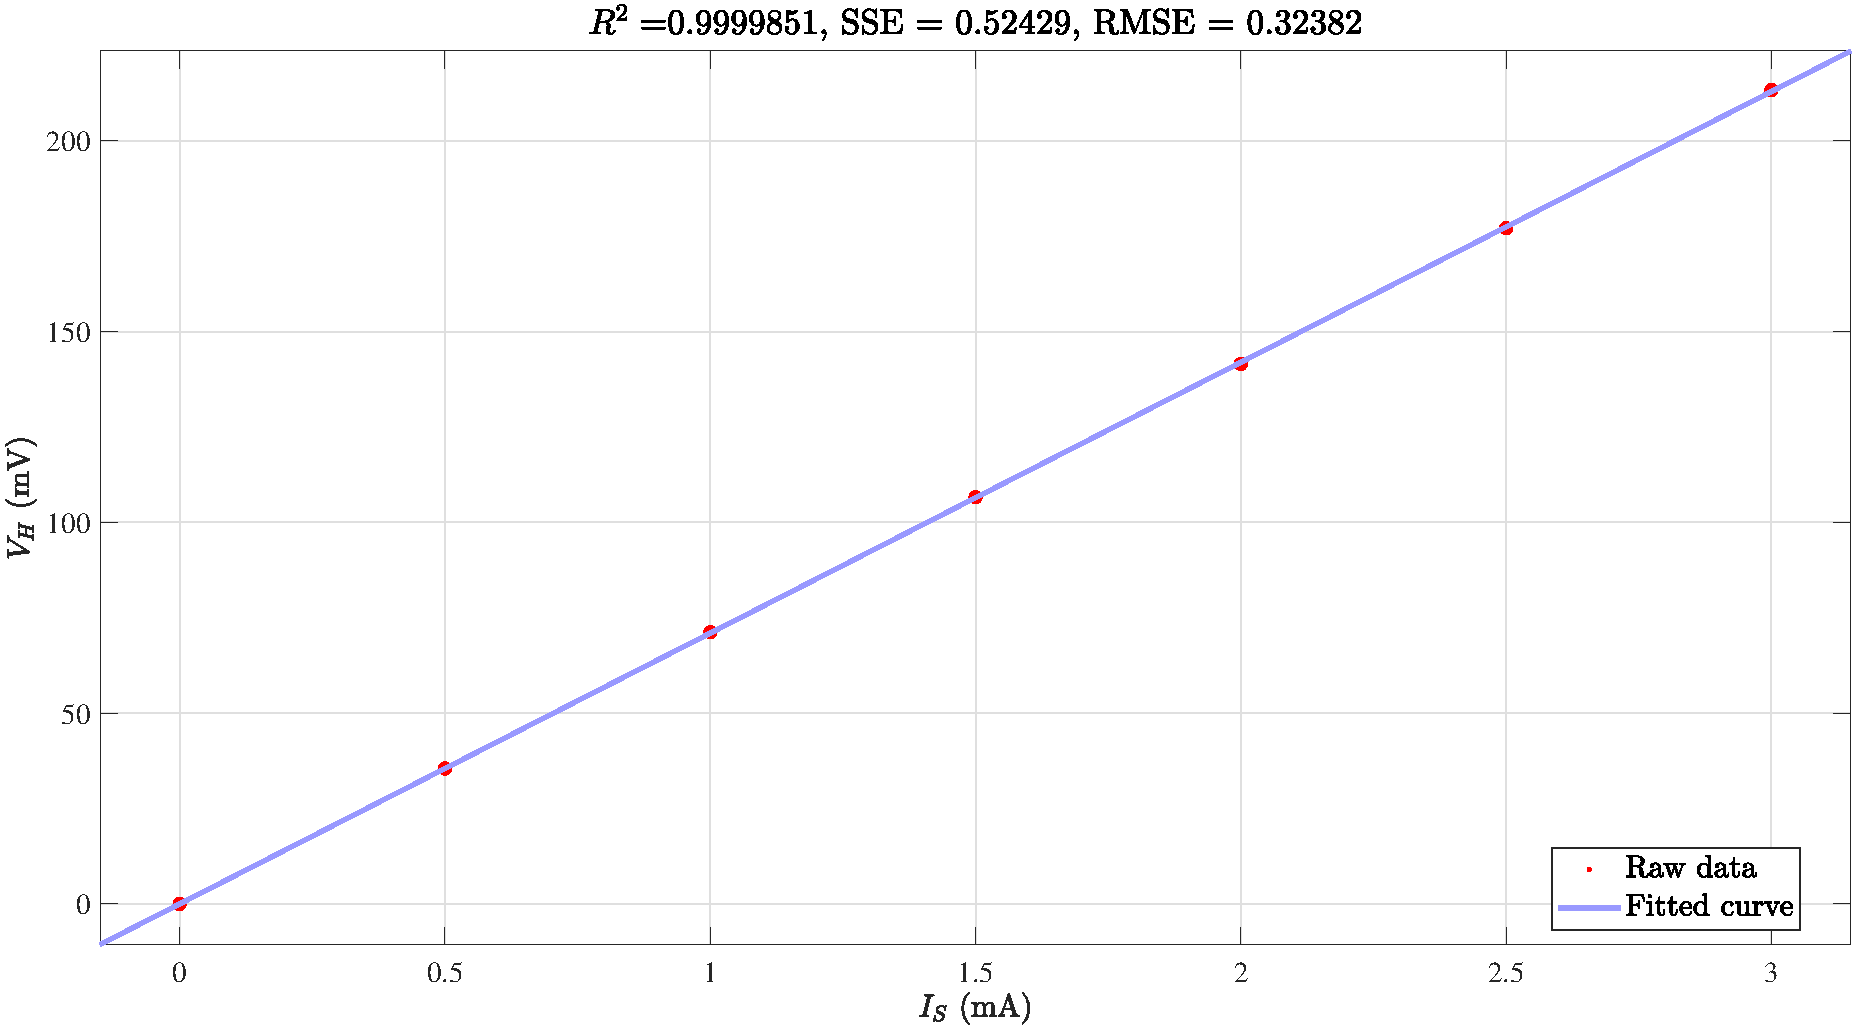
\includegraphics[width=0.9\columnwidth]{assets/1/1.pdf}
    \caption{霍尔电流 $I_S$ 与霍尔电压 $U_H$ 的关系}
    \label{霍尔电流与霍尔电压的关系 图}
\end{figure}


\subsubsection{霍尔电压 $V_H$ 与磁感应强度 $B$ 的关系、磁感应强度 $B$ 与磁励电流 $I_M$ 的关系}
设置霍尔电流保持$ I_S = 1.00 \ \mathrm{mA}$,由 1,2 端输入,将特斯拉计的探头小心地伸入电磁铁间隙中心处,调节励磁电流$ I_M $从$ 0 $至 300 mA,每隔 50 mA 分别测出磁场 $\boldsymbol{B}$ 的大小和样品的霍尔电压$ U_H $,每次消除副效应,得到结果如表 \ref{霍尔电压与磁励电流} 和表 \ref{磁感应强度与磁励电流} 所示。


在 Matlab 中,我们用最小二乘法进行拟合,如图 \ref{霍尔电压、磁感应强度与磁励电流间的关系} 所示。$V_H$-$B$ 和 $B$-$I_M$ 的拟合优度分别为:
\begin{gather}
V_H \text{-} B: \quad R^2 = 0.9999890,\quad \text{SSE} = 0.38995,\quad  \text{RMSE} = 0.27927 \\
B \text{-} I_M: \quad R^2 = 0.9999851,\quad \text{SSE} = 1.04128,\quad  \text{RMSE} = 0.45635
\end{gather}
由图和拟合优度可以知道,数据的线性性极好。
\begin{figure}[H]\centering
\begin{subfigure}[b]{0.5\columnwidth}\centering
    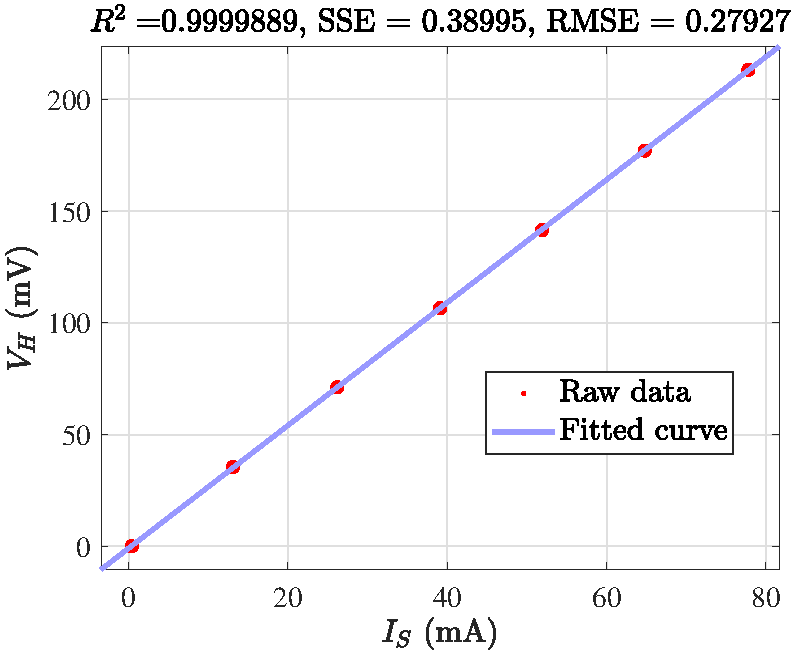
\includegraphics[height=180pt]{assets/1/2.pdf}
    \caption{霍尔电压 $V_H$ 与磁感应强度 $B$ 的关系}
\end{subfigure}\hfill
\begin{subfigure}[b]{0.5\columnwidth}\centering
    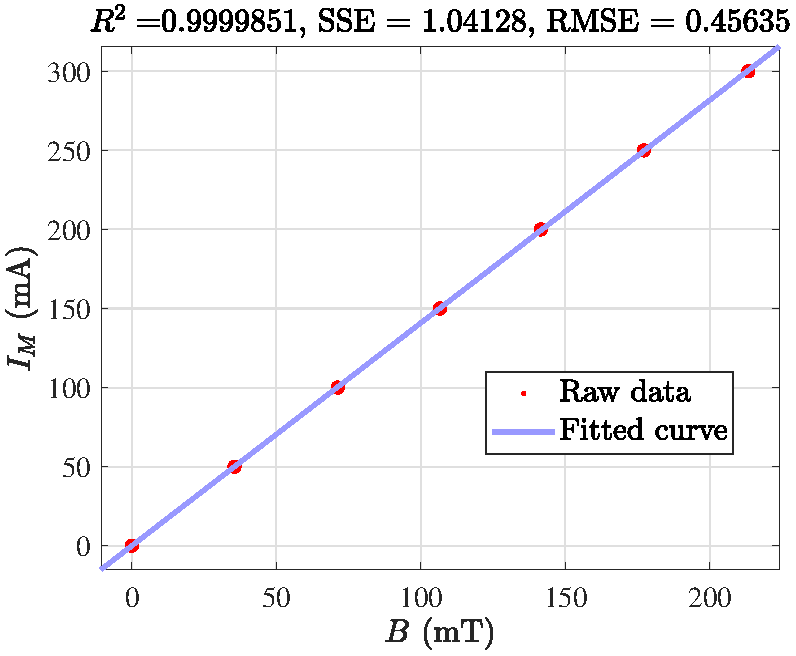
\includegraphics[height=180pt]{assets/1/3.pdf}
    \caption{磁感应强度 $B$ 与磁励电流 $I_M$ 的关系}
\end{subfigure}
\caption{霍尔电压、磁感应强度与磁励电流间的关系}
\label{霍尔电压、磁感应强度与磁励电流间的关系}
\end{figure}


\begin{table}[H]\centering
    %\renewcommand{\arraystretch}{1.5} % 调整行间距为 1.5 倍
    %\setlength{\tabcolsep}{1.5mm} % 调整列间距
    \caption{霍尔电压 $V_H$ 与磁励电流 $I_M$}
    \label{霍尔电压与磁励电流}
\begin{tabular}{cccccccccc}\toprule
    $I_M$ (mA) & $V_1$ (mV)  & $V_2$ (mV)  & $V_3$ (mV)   & $V_4$ (mV)   & $V_H$ (mV)    \\
    \midrule
    0	&-0.3	&0.3	&0.4	&-0.4	   &  0.35\\
    50	&12.4	&-12.4	&13.1	&-13.1	   & 12.75\\
    100	&25.2	&-25.2	&26.2	&-26.2	   &  25.7\\
    150	&38.3	&-38.4	&39.1	&-39.1	   &38.725\\
    200	&51.0	&-51.0	&51.9	&-51.9	   & 51.45\\
    250	&64.0	&-64.0	&64.8	&-64.8	   &  64.4\\
    300	&76.9	&-76.9	&77.7	&-77.8	   &77.325\\
    \bottomrule
\end{tabular}
\end{table}\vspace*{-2mm}
\begin{table}[H]\centering
    %\renewcommand{\arraystretch}{1.5} % 调整行间距为 1.5 倍
    %\setlength{\tabcolsep}{1.5mm} % 调整列间距
    \caption{磁感应强度 $B$ 与磁励电流 $I_M$}
    \label{磁感应强度与磁励电流}
\begin{tabular}{cccccccccc}\toprule
    $I_M$ (mA) & $B_1$ (mT)  & $B_2$ (mT)  & $B_3$ (mT)   & $B_4$ (mT)   & $B$ (mT)    \\
    \midrule
    0	&0.0	&0.0	&0.0	&0.0	    &     0\\
    50	&35.2	&35.2	&-35.6	&-35.5	    &35.375\\
    100	&70.6	&70.6	&-71.2	&-71.2	    &  70.9\\
    150	&106.5	&106.5	&-106.6	&-106.6	    &106.55\\
    200	&141.7	&141.6	&-141.5	&-141.5	    &141.57\\
    250	&177.7	&177.7	&-177.1	&-177.1	    & 177.4\\
    300	&213.4	&213.5	&-213.3	&-213.3	    &213.38\\
    \bottomrule
\end{tabular}
\end{table}



\subsubsection{计算霍尔元件的霍尔灵敏度}

依据 $V_H$-$B$ 曲线的拟合结果,拟合直线为:
\begin{equation}
B = 2.75 \,V_H - 0.8916
\end{equation}
上式中 $V_H$ 和 $B$ 的单位分别是 mV 和 mT,于是直线斜率 $k = \frac{\Delta B}{\Delta V_H} = 2.75 \ \mathrm{mT\cdot mV^{-1}}$,而霍尔电流 $I_S = 1 \ \mathrm{mA} = 0.001 \ \mathrm{A}$,可求得霍尔灵敏度:
\begin{equation}
K_H = \frac{1}{I_S k} = \frac{1}{0.001 \ \mathrm{A} \times  2.75 \ \mathrm{mT\cdot mV^{-1}}} = 363.6364 \  \  \ \mathrm{mV}\cdot \mathrm{A^{-1}}\cdot \mathrm{mT}^{-1}
\end{equation}
与实验器材上的标定值 $371 \  \  \ \mathrm{mV}\cdot \mathrm{A^{-1}}\cdot \mathrm{mT}^{-1}$ 比较,相对误差 $\eta$ 为:
\begin{equation}
\eta = \frac{K_H - 371}{371} \times 100\% = - 1.9848 \%
\end{equation}
与标准值基本符合。再计算 $K_H$ 的不确定度:
又$ R^2=0.9999889 $,那么根据不确定度公式$ \frac{\sigma_{K_H}}{K_H}=\sqrt{\frac{1-R^2}{(n-2)R^2}} $可以计算得到:
\begin{equation}
\sigma_{K_H}=K_H\sqrt{\frac{1-R^2}{(n-2)R^2}}= 0.7650 \  \  \ \mathrm{mV}\cdot \mathrm{A^{-1}}\cdot \mathrm{mT}^{-1}
\end{equation}
按不确定度的标准,向上保留为 1 位有效数字,则 $K_H$ 应写为:
\begin{equation}
K_H = 363.6\  (\pm 0.8) \  \  \ \mathrm{mV}\cdot \mathrm{A^{-1}}\cdot \mathrm{mT}^{-1}
\end{equation}



\subsubsection{电磁铁在水平方向的磁场分布}

在 $I_M = 0$ 的条件下,调零毫特计。调节 $I_M = 200 \ \mathrm{mA}$,不断调节移动尺的位置,每 2 mm 记录毫特计读数值,得到数据如表 \ref{测量电磁铁磁场沿水平方向的分布} 所示。
\begin{table}[H]\centering
    %\renewcommand{\arraystretch}{1.5} % 调整行间距为 1.5 倍
    %\setlength{\tabcolsep}{1.5mm} % 调整列间距
    \caption{测量电磁铁磁场沿水平方向的分布}
    \label{测量电磁铁磁场沿水平方向的分布}
\resizebox{\columnwidth}{!}{
    \begin{tabular}{cccccccccccccccccc}\toprule
        $X$ (mm) & 42	&40	&38	&36	&34	&32	&30 &28	&26	&24	&22	&20	&18	&16	&14 \\
        \midrule
        $B$ (mT) & 143.2	&143.3	&143.2	&143.1	&143.1	&143.1	&143.1 &143.1	&143.1	&143.1	&143.1	&143.1	&143.1	&143.1	&143.0 \\
        \bottomrule
    \end{tabular}
}
\end{table}
作出磁场分布图像如下:
\begin{figure}[H]\centering
    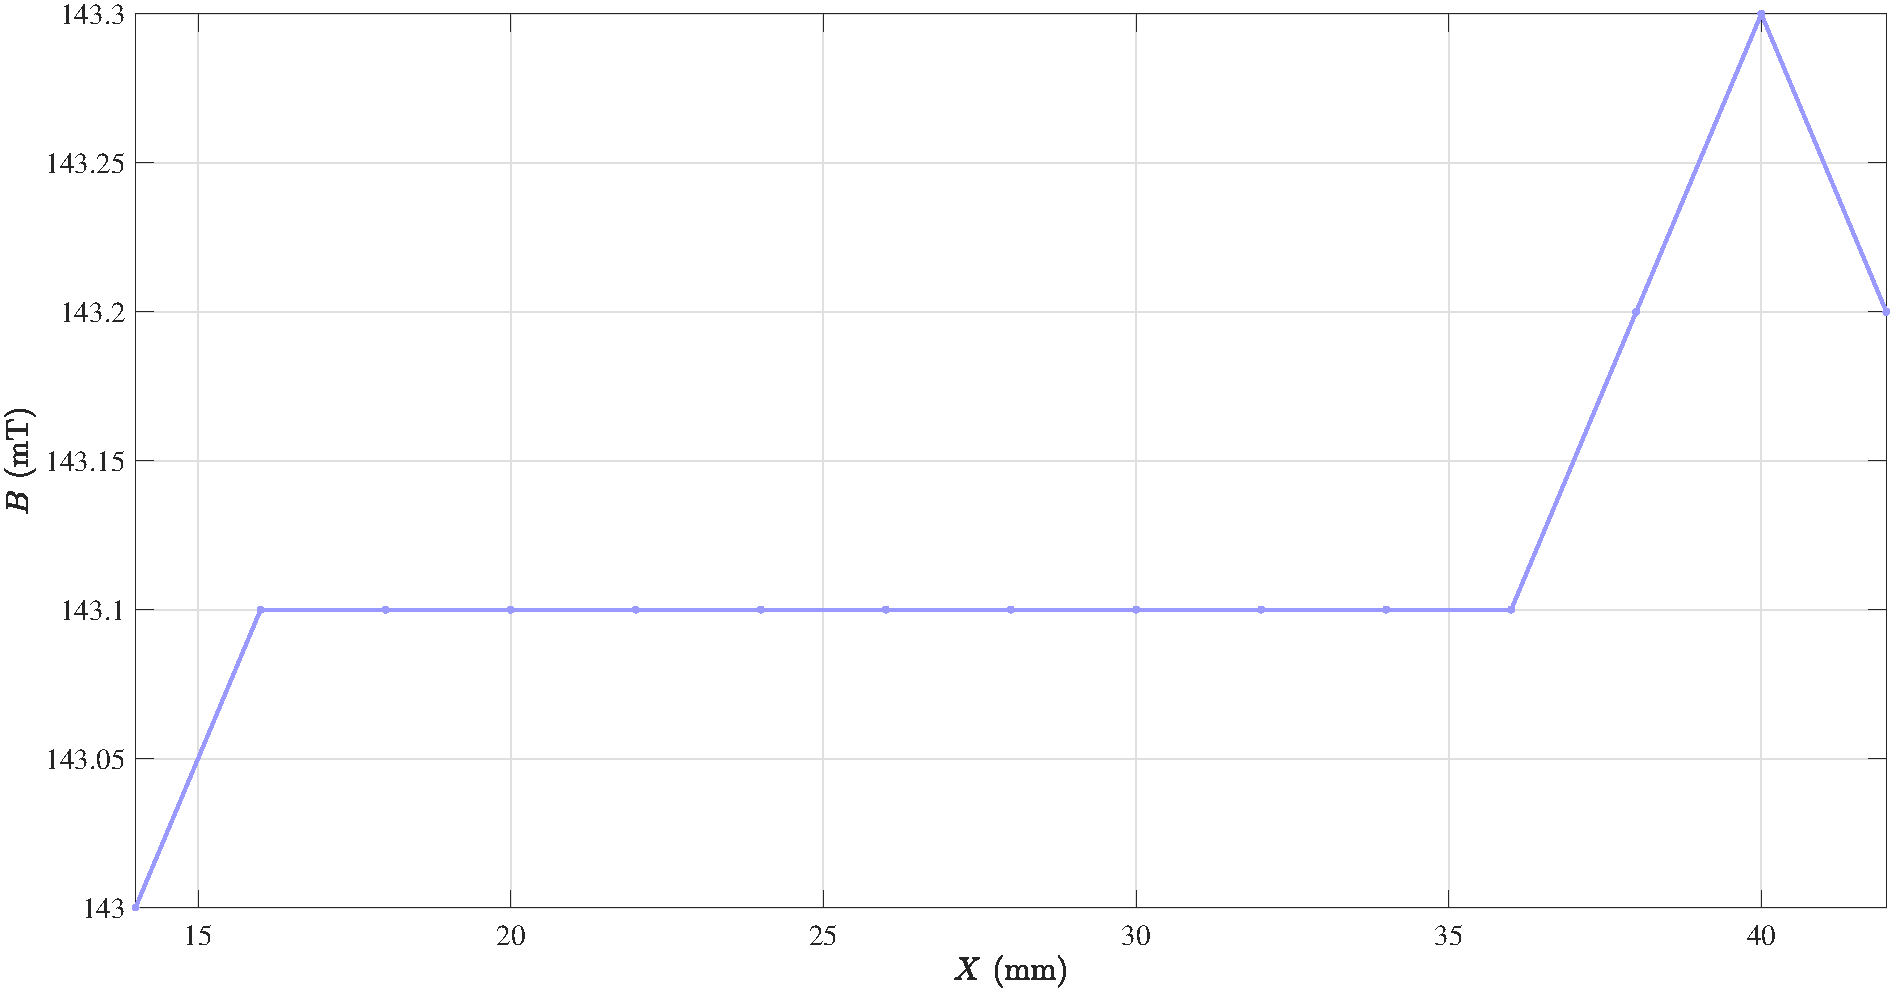
\includegraphics[width=0.9\columnwidth]{assets/1/4.pdf}
    \caption{电磁铁在水平方向的磁场分布}
\end{figure}

\subsubsection{用交流霍尔电流测磁场}
用函数发生器替代直流稳压电源,设置$ f=500\,\mathrm{Hz} $,调节输出电压使得交流霍尔电流保持$ I_{S, AC}= 1\,\mathrm{mA} $。交流霍尔电流可用多用表的交流 mA 档测量。霍尔电流设定好后,用多用表测量霍尔电压$ U_H $。电磁铁的励磁电流依次为 50 mA, 75 mA, ..., 200 mA。得到的数据见表 \ref{交流霍尔电流测磁场数据}。

\begin{table}[H]\centering
    %\renewcommand{\arraystretch}{1.5} % 调整行间距为 1.5 倍
    %\setlength{\tabcolsep}{1.5mm} % 调整列间距
    \caption{交流霍尔电流测磁场数据}
    \label{交流霍尔电流测磁场数据}
\begin{tabular}{cccccccccc}\toprule
    $I_M$ (mA) &50	    &75	    &100	&125	&150	&175	&200    \\
    \midrule
    $B$ (mT) & 34.9	&52.6	&70.5	&88.4	&106.1	&124.0	&141.4  \\
    $V_{H, AC}$ (mV) & 14.530	&21.499	&28.503	&35.694	&42.795	&50.013	&56.814 \\
    \bottomrule
\end{tabular}
\end{table}
作出$ B$-$I_M $图像如下:
\begin{figure}[H]\centering
    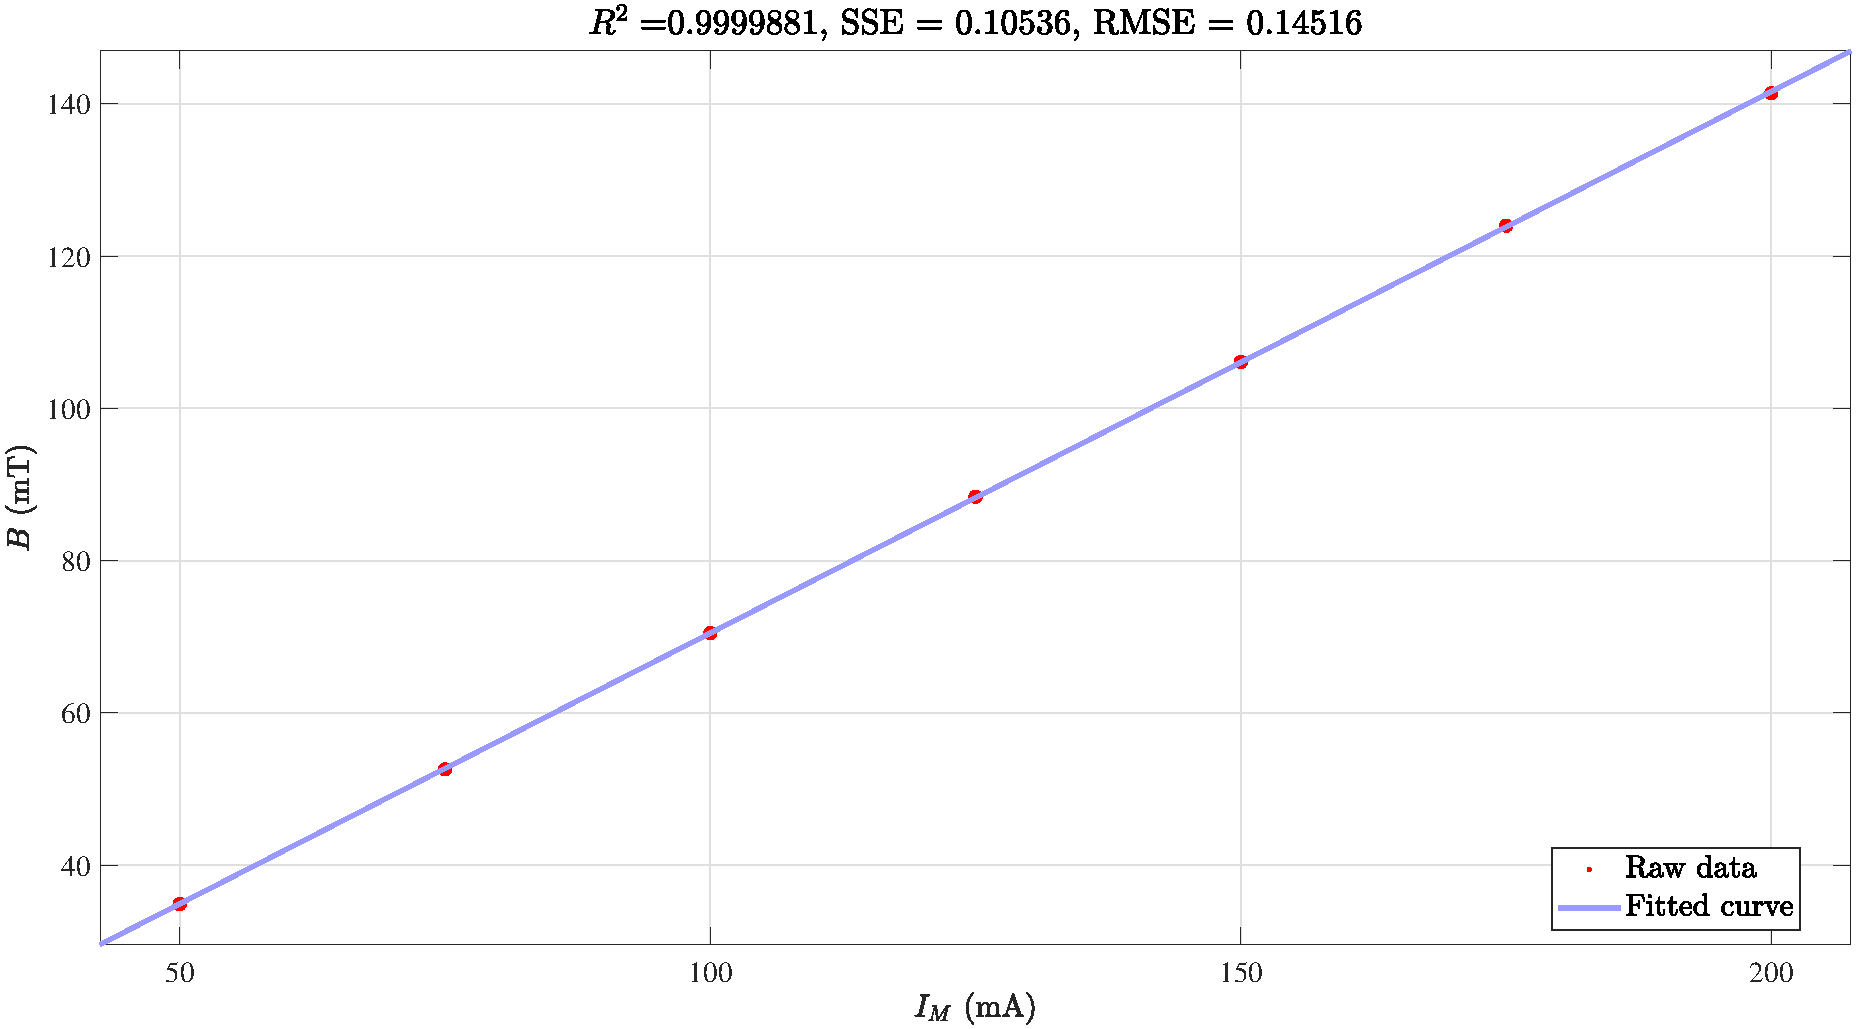
\includegraphics[width=0.9\columnwidth]{assets/1/5.pdf}
    \caption{AC 模式下磁感应强度 $B$ 随磁励电流 $I_M$ 的变化}
\end{figure}


\section{第二部分:亥姆霍兹线圈的磁场测量}


\subsection{实验目的}
\begin{enumerate}
\item 掌握载流圆线圈的磁场分布;
\item 掌握亥姆霍兹线圈的磁场分布。
\end{enumerate}


\subsection{实验仪器与用具}
亥姆霍兹线圈磁场实验仪由亥姆霍兹线圈架部分和磁场测量仪组成。亥姆霍兹线圈架部分包括有一个传感器盒,里面装有用于测量磁场的感应线圈。主要技术指标如下:

\begin{enumerate}
\item 亥姆霍兹线圈架:两个励磁线圈线圈有效半径 105\,mm,单个线圈匝数400匝,两线圈中心间距105\,mm;移动装置轴向可移动距离250\,mm,径向可移动距离70\,mm,距离分辨率1\,mm ;探测线圈匝数 1000,旋转角度$ 360\,^\circ $
\item DH4501 亥姆霍兹磁场测量仪: 频率范围:= $ 20\sim 200\,\mathrm{Hz} $,频率分辨率:$ 0.1\,\mathrm{Hz} $,测量误差 0.1\%;正弦波输出电压幅度最大$ 20\, $Vp-p,输出电流幅度最大 200\,mA;数显毫伏表电压测量范围 $ 0\sim 20\,\mathrm{mV} $,测量误差1\%;
\item 电源:$ 220\,\mathrm V\pm 10\% $
\item 外形尺寸:亥姆霍兹线圈架$ 340\,\mathrm{mm}\times270\,\mathrm{mm}\times250\,\mathrm{mm} $,磁场测试仪$ 320\,\mathrm{mm}\times300\,\mathrm{mm}\times120\,\mathrm{mm} $
\end{enumerate}


\subsection{实验原理}
\subsubsection{载流圆线圈和亥姆霍兹线圈的磁场}

\noindent \textbf{载流圆线圈的磁场:}\par
一半径为$ R $,通以电流$ I $的圆线圈,其轴线上磁场的公式为
\begin{equation}
B = \frac{\mu_0 N_0 I_0}{2}\cdot \frac{R^2}{\left(R^2 + x^2\right)^{\frac{3}{2}}}
\end{equation}
其中$ N_0 $为该圆线圈的匝数,$ x $为轴上某一点到圆心$ O $的距离,$ \mu_0=4\pi\times10^{-7}\,\mathrm{H/m} $。轴线磁场分布如下:

\begin{figure}[H]
    \centering
    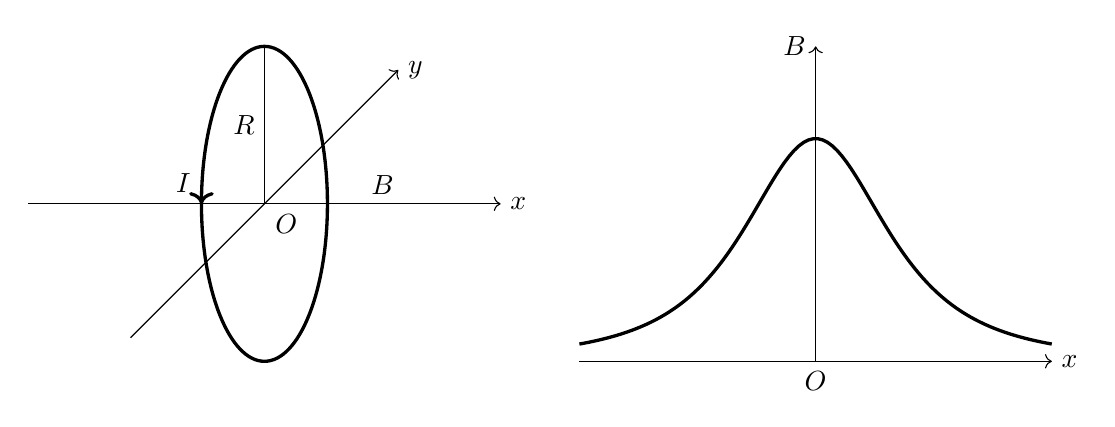
\begin{tikzpicture}
        \draw[very thick] (0,0)node[below right]{$ O $} ellipse (0.8 and 2);
        \draw[very thick,->] (-0.8,0.1)--(-0.8,0)node[above left]{$ I $};
        \draw[->] (-3,0)--(3,0)node[right]{$ x $};
        \draw (0,0)--node[left,midway]{$ R $}(0,2);
        \draw[->] (-1.7,-1.7)--(1.7,1.7)node[right]{$ y $};
        \node[above] at(1.5,0) {$ B $};
        
        \draw[->] (4,-2)--(10,-2)node[right]{$ x $};
        \draw[->] (7,-2)node[below]{$ O $}--(7,2)node[left]{$ B $};
        \draw[very thick, domain=4:10,samples=100] plot (\x,{16/(2*pow(2+pow(\x-7,2),1.5))-2});
    \end{tikzpicture}
    \caption{载流圆线圈轴向磁场分布}
\end{figure}

本实验取$ N_0=400 $匝,$ R=105\,\mathrm{mm} $。当$ f=120\,\mathrm{Hz},\;I=60\,\mathrm{mA} $\footnote{此部分实验所用$ I $均为有效值。},圆心处$ X=0 $,可计算得到单个圆线圈中的磁感应强度约为$ B=0.144\,\mathrm{mT} $.

~\\
\noindent \textbf{亥姆霍兹线圈的磁场:}\par
所谓亥姆霍兹线圈彼此平行且共轴,使得线圈上通以相同方向的电流$ I $。理论计算可证明:当线圈距离$ a $等于线圈半径$ R $时,两个单线圈的磁场叠加在轴(两个线圈的圆心连线)上中点附近较大范围内的和磁场是均匀的,如下图:

设$ z $为亥姆霍兹线圈中轴线上某一点离中心点$ O $的距离,则亥姆霍兹线圈上该点的磁感应强度为
\begin{gather}
B=\frac12\mu_0NIR^2\left\{\left[R^2+\left(z + \frac{a}{2}\right)^2\right]^{-3/2}+\left[R^2+\left(z - \frac{a}{2}\right)^2\right]^{-3/2}\right\} \\ 
\overset{a = R}{\Longrightarrow}
B=\frac12\mu_0NIR^2\left\{\left[R^2+\left(z + \frac{R}{2}\right)^2\right]^{-3/2}+\left[R^2+\left(z - \frac{R}{2}\right)^2\right]^{-3/2}\right\} 
\end{gather}
而在亥姆霍兹线圈轴线上中心$ O $点处,$ z=0 $,则该处磁感应强度为
\begin{equation}
B=\frac{\mu_0N_0I}{2R}\times\frac{16}{5^{3/2}}
\end{equation}
实验中取$ N_0=400 $匝,$ R=105\,\mathrm{mm} $。当$ f=120\,\mathrm{Hz},\;I=60\,\mathrm{mA} $时,在中心$ O $处$ z=0 $,可计算得到亥姆霍兹线圈(两个线圈的合成)磁感应强度为
\begin{equation}
B=\frac{\mu_0N_0I}{2R}\times\frac{16}{5^{3/2}}=2.05\,\mathrm{mT}
\end{equation}

\newpage
\subsubsection{电磁感应法测磁场}
\noindent \textbf{电磁感应法测量原理:}\par
对于由正弦交流信号驱动的线圈产生的交变磁场,其磁场强度的瞬时值为
\begin{equation}
B=B_{\max}\sin\omega t
\end{equation}

其中$ B_{\max} $为磁感应强度的峰值,其有效值为 $\boldsymbol{B}$ ,$ \omega $为角频率。磁场中一探测线圈的磁通量为
\begin{equation}
\Phi=NSB_{\max}\cos\theta\sin\omega t
\end{equation}
其中$ N $为探测线圈的匝数,$ S $为该线圈的截面积,$ \theta $为 $\boldsymbol{B}$ 方向与线圈法线的夹角。线圈产生的感应电动势为
\begin{equation}
\varepsilon=-\frac{\mathrm{d}\Phi}{\mathrm{d} t}=NS\omega B_{\max}\cos\theta\cos\omega t=-\varepsilon_{\max}\cos\omega t
\end{equation}
其中$ \varepsilon_{\max}=NS\omega B_{\max}\cos\theta $是线圈法线和磁场成$ \theta $角时感应电动势的幅值。当$ \theta=0^\circ,\;\varepsilon_{\max}=NS\omega B_{\max} $,此时感应电动势的幅值最大。如果用数字毫伏表测量此时线圈的电动势,则毫伏表的示数(即有效值)$ U_{\max} $为$ \frac{\varepsilon_{\max}}{\sqrt 2} $,则
\begin{equation}
B_{\max}=\frac{\varepsilon_{\max}}{NS\omega}=\frac{\sqrt 2U_{\max}}{NS\omega}
\end{equation}

~\\
\noindent \textbf{探测线圈的设计:}\par
实验中由于磁场的不均匀性,而探测线圈又无法做到很小,否则会影响测量灵敏度。一般设计的线圈长度$ L $和外径$ D $有关系$ L=\frac23D $,线圈内径$ d $与外径$ D $有关系$ d\leq\frac3D $。线圈在磁场中的等效面积为
\begin{equation}
S=\frac{13}{108}\pi D^2
\end{equation}
这样的线圈测得的平均磁感强度可以近似看成是中心点的磁感应强度。本实验励磁电流由专用的交变磁场测试仪提供。
\begin{equation}
B=\frac{54}{13\pi^2ND^2f}U_{\max}
\end{equation}
将不同的频率$ f $代入上式即可计算得到 $\boldsymbol{B}$ ,本实验$ D=0.012\,\mathrm m,\;N=1000 $匝。

\subsection{实验内容与实验步骤}
\subsubsection{测量圆电流线圈轴线上的磁场分布}
调节频率调节电位器,使得频率表读数为$ 120\,\mathrm{Hz} $。调节磁场实验仪的电流调节电位器使得励磁电流有效值为$ I=60\,\mathrm{mA} $,以圆电流线圈中心为坐标原点,每隔5\,mm测一个$ U_{\max} $值,测量过程中注意保持励磁电流值不变,保证探测线圈法线方向与圆电流线圈轴线的夹角为$ 0^\circ $.
\subsubsection{测量亥姆霍兹线圈轴线上的磁场分布}
在励磁电流为零的情况下将磁感应强度清零。将磁场实验仪的两个线圈串联接入交流电场,调节频率电位器使得频率表读数为120\,Hz,调节磁场测量仪的电流调节电位器使得励磁电流有效值为60\,mA。以亥姆霍兹线圈中心为坐标原点,每隔5\,mm测一磁感应强度$ U_{\max} $的值,测量过程中注意保持励磁电流值不变。
\subsubsection{测量亥姆霍兹线圈沿径向的磁场分布}
固定探测线圈法线方向和圆电流轴线$ D $的夹角为$ 0^\circ $,转动探测线圈径向移动手轮,每隔5\,mm测量一个数据,按正负方向测到边缘,记录数据并作出磁场分布曲线图。
\subsubsection{线圈转角与感应电压的关系}
当$ NS\omega B_{\max} $不变时,$ \varepsilon_{\max} $与$ \cos\theta $成正比。根据实验要求,将探测线圈沿轴线固定在某一位置上,让探测线圈法线方向与圆电流轴线的夹角从$ 0^\circ $开始,逐步转移到$ 90^\circ,\;180^\circ,\;270^\circ $,再回到$ 0^\circ $,每改变$ 10^\circ $测量一组数据。
\subsubsection{励磁电流频率大小对磁场强度的影响}
将探测线圈固定在亥姆霍兹线圈中心点,其法线方向与圆电流轴线$ D $夹角为$ 0^\circ $,并保持不变。调节磁场测试仪输出电流频率,在$ 20\sim 130\,\mathrm{Hz} $范围内,每次频率改变$ 10\,\mathrm{Hz} $,逐次测量感应电动势的数值并记录。

\subsection{实验结果与数据处理}
\subsubsection{圆线圈轴线上的磁场分布}
将单个圆电流线圈接入电路,轴向移动探测线圈记录不同位置下的$ U_{\max} $,依据原始数据,计算得到磁感应强度 $B$ 的大小,如下表所示:

\begin{table}[H]\centering
    %\renewcommand{\arraystretch}{1.5} % 调整行间距为 1.5 倍
    %\setlength{\tabcolsep}{1.5mm} % 调整列间距
    \caption{圆线圈轴线上的磁场分布}
    \label{圆线圈轴线上的磁场分布}
\resizebox{\columnwidth}{!}{
    \begin{tabular}{cccccccccccccccc}\toprule
        距离 $X$ (mm) &-25	 &-20	       &-15	        &-10	       & -5	            &0	            &5	            &10	            &15	            &20	            &25\\
        \midrule
        $U_{\max}$ (mV) &5.45	 &5.62	       &5.75	    &5.83	       & 5.88	        &5.90	        &5.88	        &5.81	        &5.70	        &5.58	        &5.41\\
        $B_{\text{theoretical}}$ (mT) &0.13289 &0.13703	   &0.1402	    &0.14215	   & 0.14337	    &0.14386	    &0.14337	    &0.14167	    &0.13898	    &0.13606	    &0.13191\\
        $B_{\text{experimental}}$ (mT) &0.13222 &0.13614	   &0.13933	    &0.14168	   & 0.14313	    &0.14362	    &0.14313	    &0.14168	    &0.13933	    &0.13614	    &0.13222\\
        \bottomrule
    \end{tabular}
}
\end{table}
根据上表数据,在同一坐标系中作出实验值与理论值的图像,如下:
\begin{figure}[H]\centering
    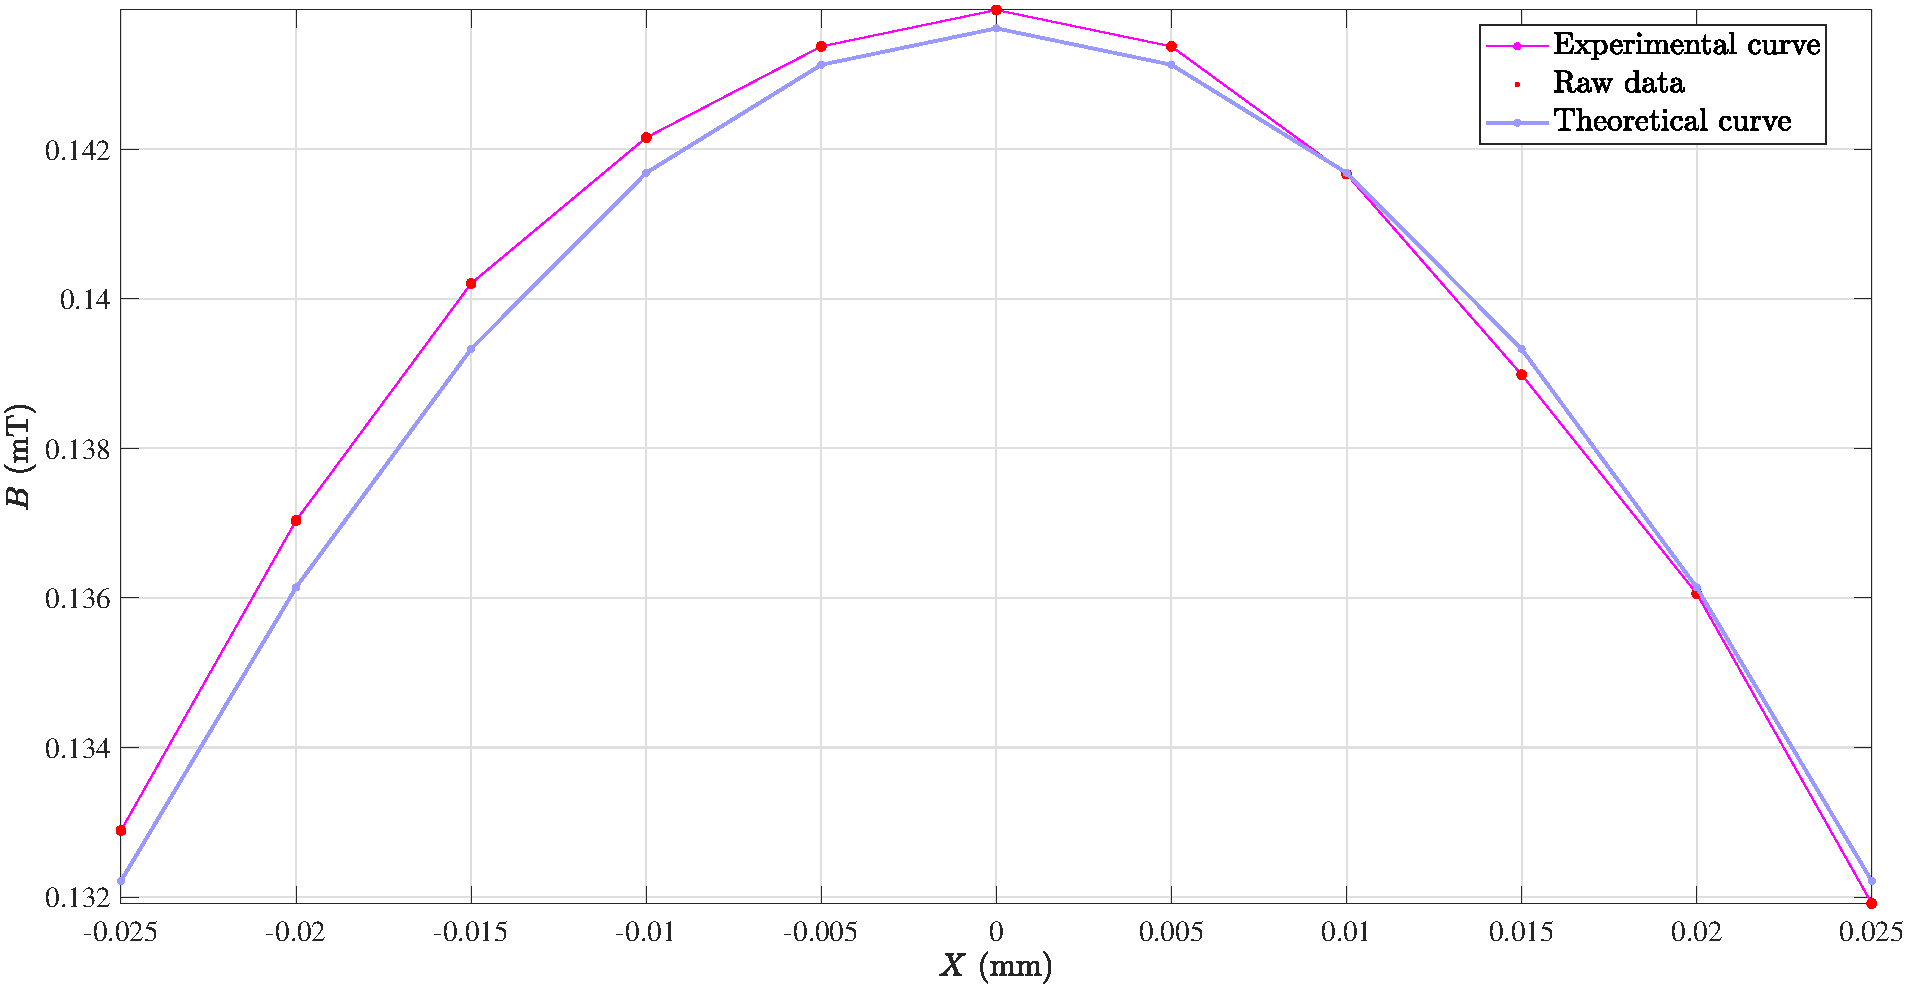
\includegraphics[width=0.9\columnwidth]{assets/2/6.pdf}
    \caption{圆线圈轴线上的磁场分布}
\end{figure}


由上图可以看出测量值与计算值随轴向位置的变化趋势大致相同,在具体数值上测量值较计算值更大。可能的原因是探测线圈或励磁线圈的实际性能由于损耗与已知参数不同,进而得到差异较大的结果。

\subsubsection{亥姆霍兹线圈轴线上的磁场分布}
实验数据记录如下:

\begin{table}[H]\centering
    %\renewcommand{\arraystretch}{1.5} % 调整行间距为 1.5 倍
    %\setlength{\tabcolsep}{1.5mm} % 调整列间距
    \caption{亥姆霍兹线圈轴线上的磁场分布}
    \label{亥姆霍兹线圈轴线上的磁场分布}
\resizebox{\columnwidth}{!}{
    \begin{tabular}{cccccccccccccccccc}\toprule
        轴向距离 $X$ (mm)&-25	    &-20	        &-15	       &-10	        &-5	            &0	            &5	            &10	    &15	    &20	&25\\
        \midrule
        $U_{\max}$ (mV) &8.43	    &8.45	        &8.46	       &8.47	    &8.46	        &8.46	        &8.46	        &8.43	&8.44	&8.44	&8.43\\
        $B_{\text{experimental}}$ (mT) &0.20555    &0.20604	    &0.20628	   &0.20653	    &0.20628	    &0.20628	    &0.20628	    &0.20555&0.2058	&0.2058	   & 0.20555\\
        \bottomrule
    \end{tabular}
}
\end{table}
在 Matlab 中,选定拟合函数为:
\begin{gather}
    B=\frac12\mu_0NIR^2\left\{\left[R^2+\left(x - x_0 + \frac{a}{2}\right)^2\right]^{-3/2}+\left[R^2+\left(x - x_0 - \frac{a}{2}\right)^2\right]^{-3/2}\right\}
\end{gather}
其中 $a$ 和 $x_0$ 为待定常量,前者是亥姆霍兹线圈之间的距离,后者是磁场中心与物理中心的偏移量,$x$ 为自变量。代入已知参数进行化简,得到:
\begin{equation}
B = 0.16625308\ \left\{ \left[ 0.011025 + \left(x - x_0 + \frac{a}{2}\right)^2\right]^{-\frac{3}{2}} + \left[ 0.011025 + \left(x - x_0 - \frac{a}{2}\right)^2\right]^{-\frac{3}{2}} \right\} \times 10^{-6}\quad (T)
\end{equation}
上式中 $x$、$x_0$ 和 $a$ 的单位都是 m,磁感应强度 $B$ 的单位是 T 。进行拟合,得到拟合结果及其优度:
\begin{gather}
a = 0.1044 \ \mathrm{m},\quad b = 0.001295 \ \mathrm{m} \\ 
R^2 = 0.2593,\quad \text{RMSE} = 3.254\times 10^{-7},\quad \text{SSE} = 9.528\times 10^{-13}
\end{gather}
$a = 104.4 \ \mathrm{mm}$ 与仪器上的标准值 $R = 105 \ \mathrm{mm}$ 十分接近,相对误差为:
\begin{equation}
\eta = \frac{a - R}{R} \times 100 \%  -0.57\%
\end{equation}
在同一坐标系下,作出拟合曲线与实验数据,由图也可以看出实验结果与实验原理中预期结果大致相符。
\begin{figure}[H]\centering
    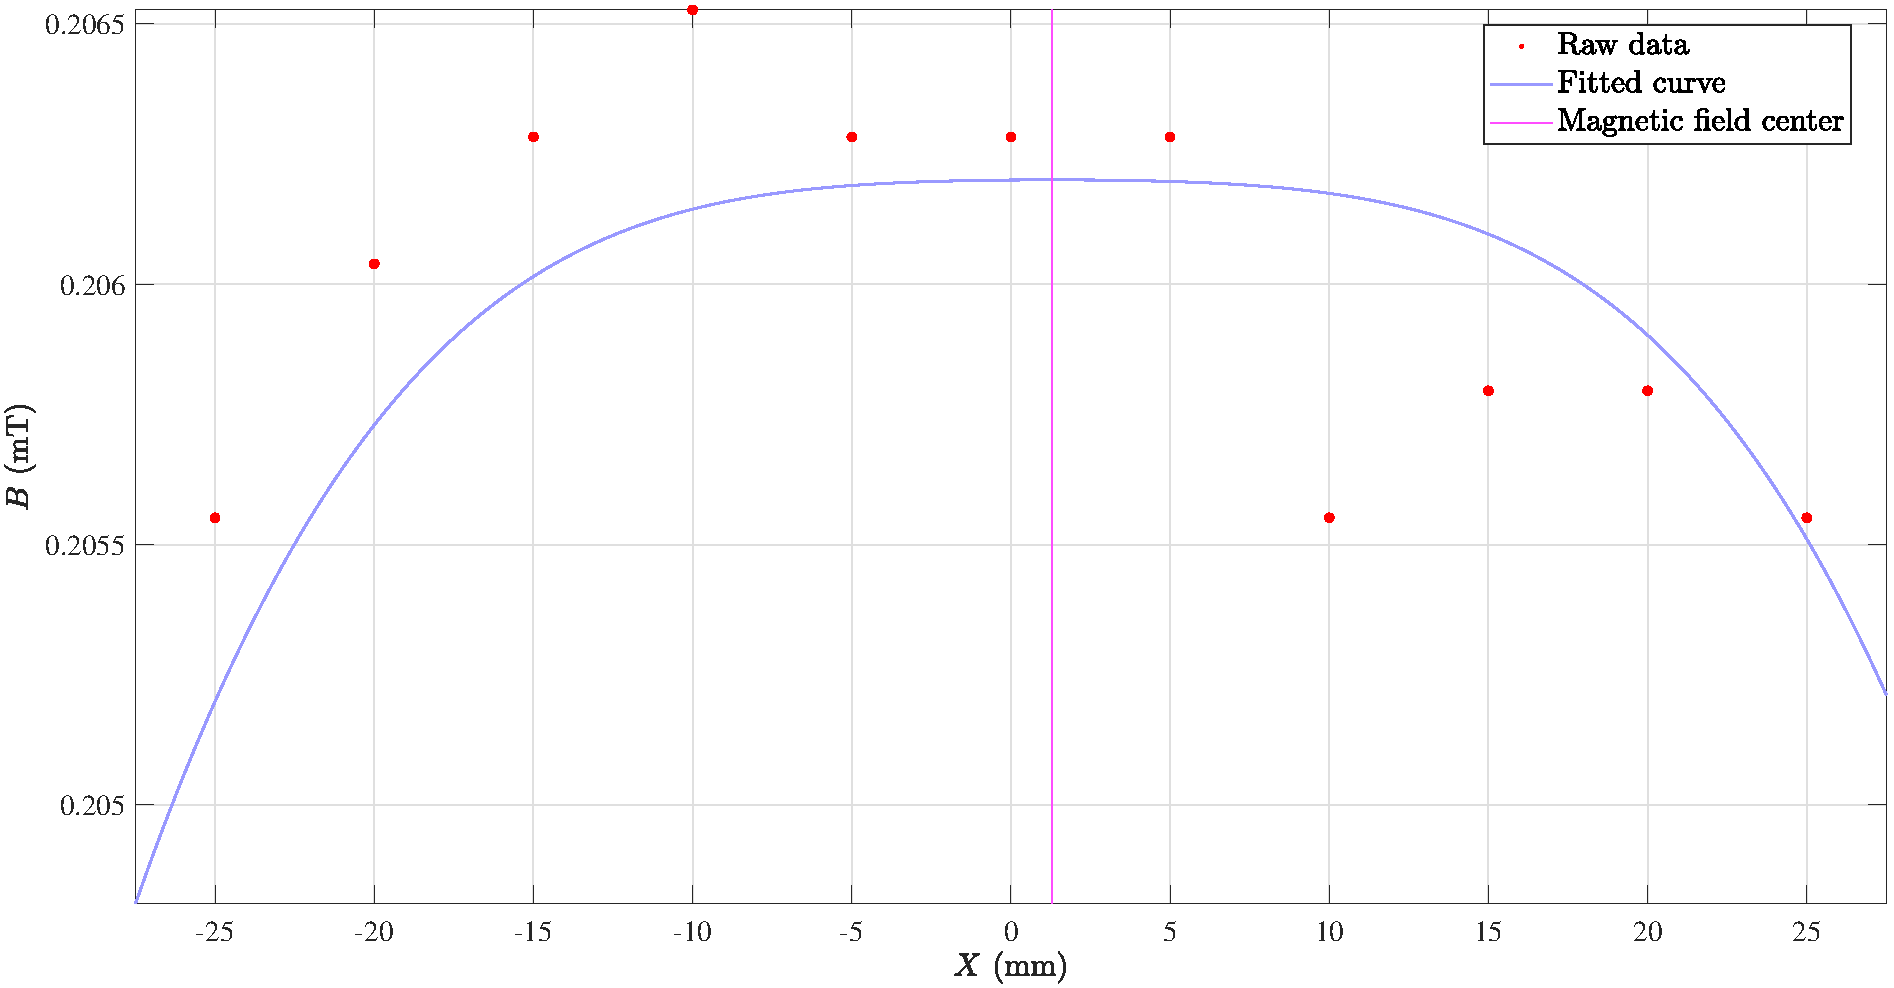
\includegraphics[width=0.9\columnwidth]{assets/2/7.pdf}
    \caption{亥姆霍兹线圈轴线上磁场分布的拟合结果}
\end{figure}

\subsubsection{测量亥姆霍兹线圈沿径向的磁场分布}
实验数据记录如下:
\begin{table}[H]\centering
    %\renewcommand{\arraystretch}{1.5} % 调整行间距为 1.5 倍
    %\setlength{\tabcolsep}{1.5mm} % 调整列间距
    \caption{亥姆霍兹线圈的径向磁场分布}
    \label{亥姆霍兹线圈的径向磁场分布}
\resizebox{\columnwidth}{!}{
    \begin{tabular}{cccccccccccccccccccccccccc}\toprule
        径向距离 $X$ (mm)&-25	&-20	&-15	&-10	&-5	&0	&5	&10	&15	&20	&25\\
        \midrule
        $U_{\max}$ (mV) &8.46	        &8.47	        &8.47	        &8.47	        &8.47	        &8.46	        &8.46	&8.46	&8.45	&8.43	&8.42\\
        $B_{\text{experimental}}$ (mT) &0.20628	    &0.20653	    &0.20653	    &0.20653	    &0.20653	    &0.20628	    &0.20628	    &0.20628	    &0.20604	    &0.20555	    &0.20531\\
        \bottomrule
    \end{tabular}
}
\end{table}
根据上表数据可作出$ B-X $曲线,如图 \ref{亥姆霍兹线圈径向磁场分布}。强度较为稳定,而离开这一定范围后磁场范围将迅速减小。
\begin{figure}[H]\centering
    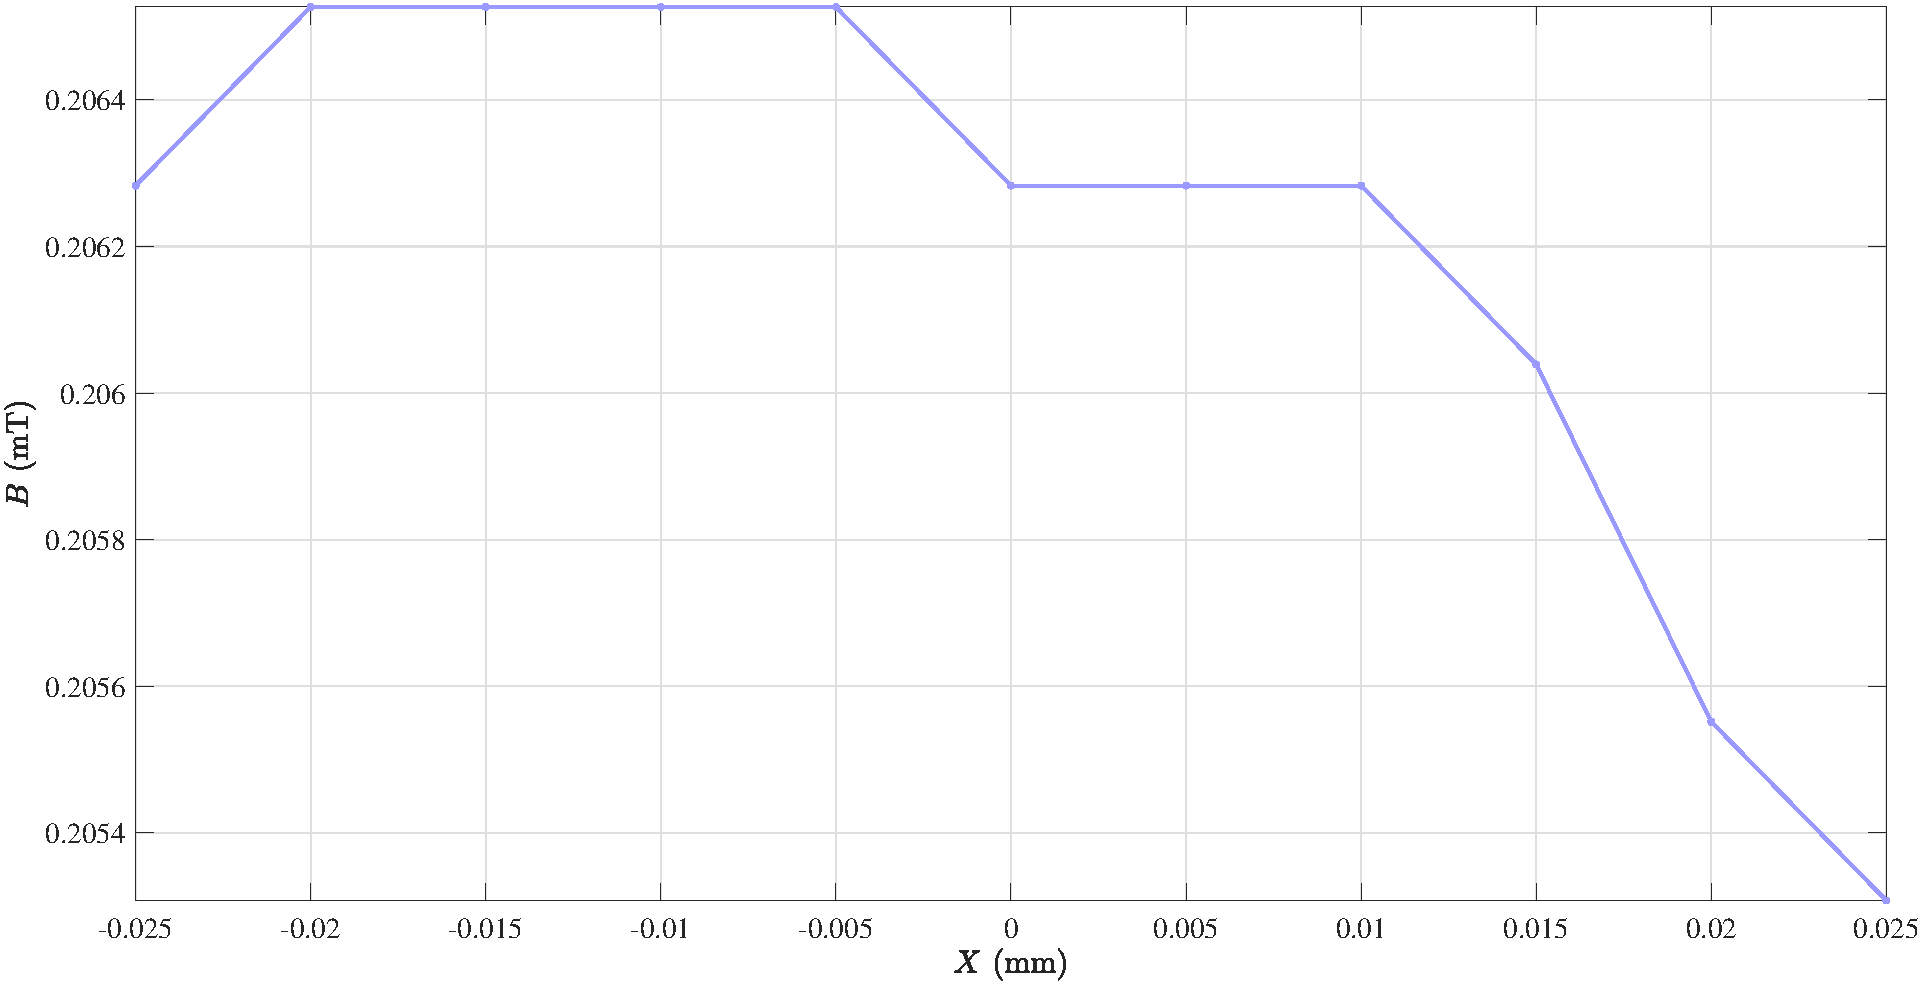
\includegraphics[width=0.9\columnwidth]{assets/2/8.pdf}
    \caption{亥姆霍兹线圈径向磁场分布}
    \label{亥姆霍兹线圈径向磁场分布}
\end{figure}
由图可以看出亥姆霍兹线圈径向磁场分布与轴向分布类似,在磁场中点附近一定范围内磁场

\subsubsection{线圈转角与感应电压的关系}
本小节验证公式 $ \varepsilon_{\max}=NS\omega B_{\max}\cos\theta $,实验数据记录如下:
\begin{table}[H]\centering
    %\renewcommand{\arraystretch}{1.5} % 调整行间距为 1.5 倍
    %\setlength{\tabcolsep}{1.5mm} % 调整列间距
    \caption{线圈转角与感应电压的关系}
    \label{线圈转角与感应电压的关系}
\begin{tabular}{|ccc|ccc|ccc|}\toprule
    $\theta$ ($^\circ$) & $U_{\text{expe}}$ (mV) & $U_{\text{theo}}$ (mV) & $\theta$ ($^\circ$) & $U_{\text{expe}}$ (mV) & $U_{\text{theo}}$ (mV) & $\theta$ ($^\circ$) & $U_{\text{expe}}$ (mV) & $U_{\text{theo}}$ (mV)   \\
    \midrule
    0	    &8.47	    &  8.47	&120	&4.01	   &  4.235	&240	&4.37	   &  4.235 \\
    10	    &8.36	    &8.3413	&130	&5.18	   & 5.4444	&250	&3.26	   & 2.8969 \\
    20	    &7.99	    &7.9592	&140	&6.30	   & 6.4884	&260	&1.74	   & 1.4708 \\
    30	    &7.38	    &7.3352	&150	&7.15	   & 7.3352	&270	&0.20	   &      0 \\
    40	    &6.59	    &6.4884	&160	&7.82	   & 7.9592	&280	&1.18	   & 1.4708 \\
    50	    &5.51	    &5.4444	&170	&8.28	   & 8.3413	&290	&2.81	   & 2.8969 \\
    60	    &4.32	    & 4.235	&180	&8.42	   &   8.47	&300	&4.27	   &  4.235 \\
    70	    &2.97	    &2.8969	&190	&8.35	   & 8.3413	&310	&5.48	   & 5.4444 \\
    80	    &1.68	    &1.4708	&200	&7.97	   & 7.9592	&320	&6.54	   & 6.4884 \\
    90	    &0.19	    &     0	&210	&7.43	   & 7.3352	&330	&7.35	   & 7.3352 \\
    100	&1.16	    &1.4708	&220	&6.78	   & 6.4884	&340	&7.98	   & 7.9592 \\
    110	&2.63	    &2.8969	&230	&5.68	   & 5.4444	&350	&8.36	   & 8.3413 \\
    \bottomrule
\end{tabular}
\end{table}
根据上表数据,在同一坐标系中作出理论值和实际值,如图 \ref{线圈转角与感应电压的关系} 所示。由图像可知,实验测量值与理论计算值重合程度较高,在误差允许范围内可看作$ U=U_{\max}\cos\theta $,即验证了$ \varepsilon_{\max}\propto\cos\theta $。
\begin{figure}[H]\centering
    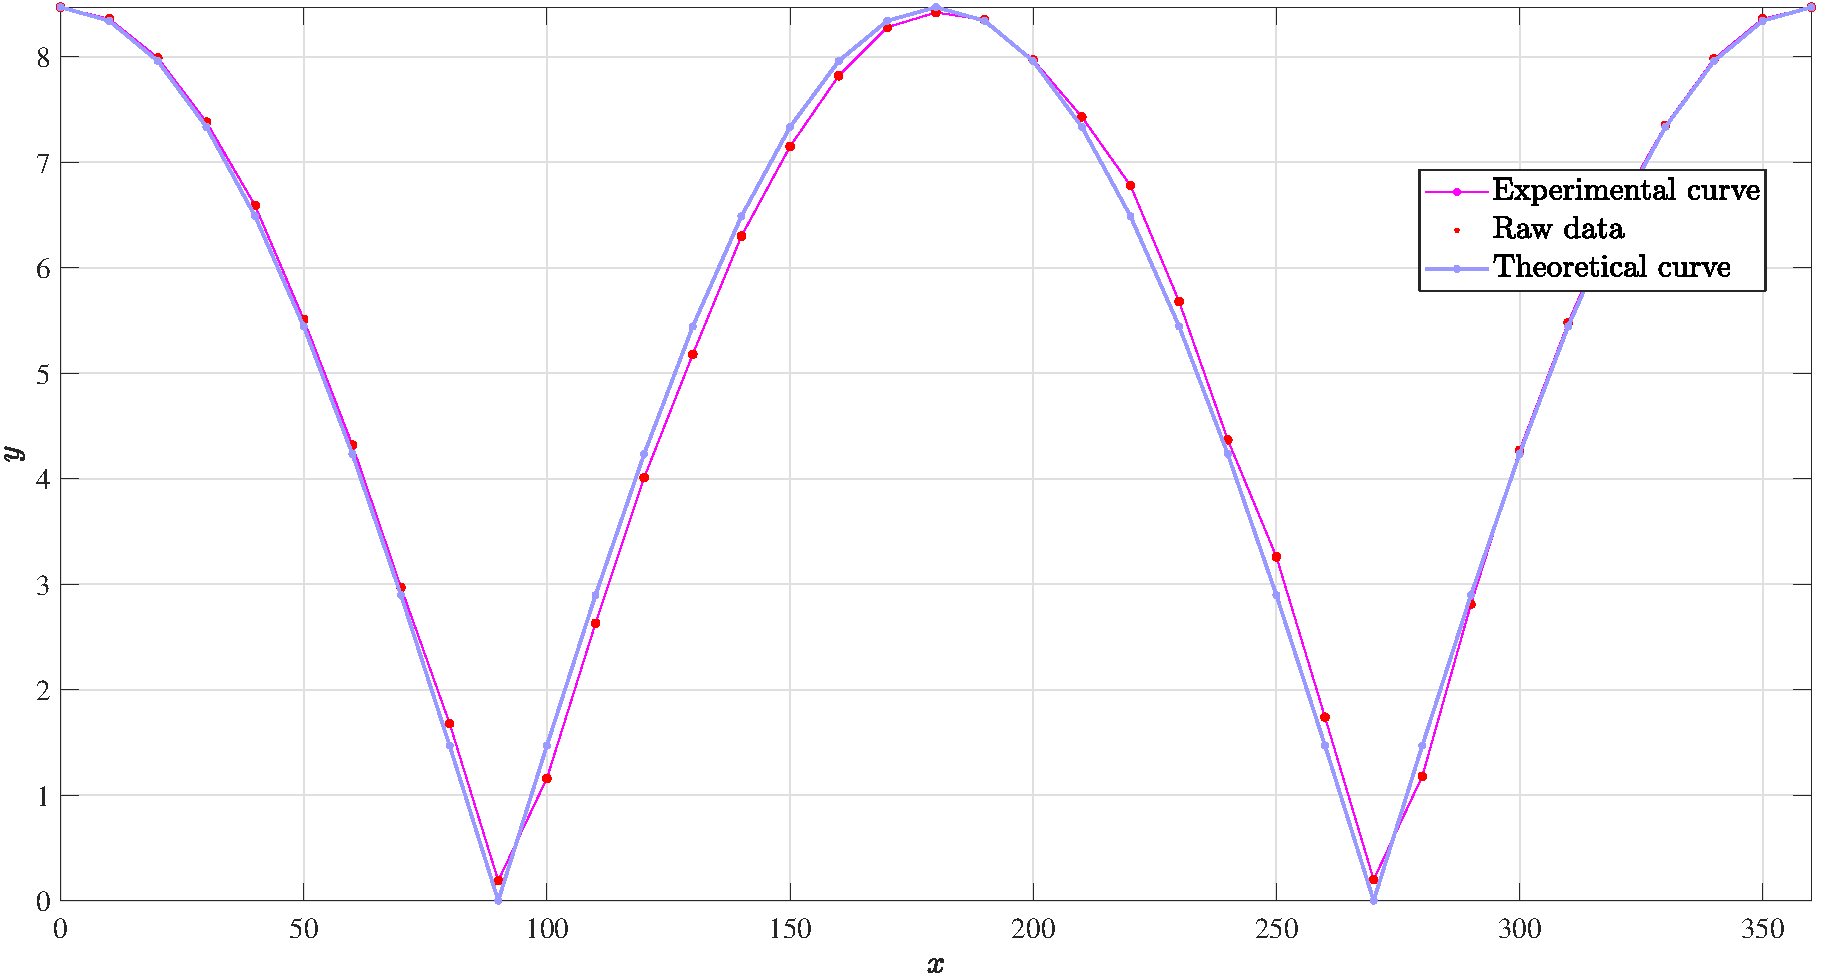
\includegraphics[width=0.9\columnwidth]{assets/2/9.pdf}
    \caption{线圈转角与感应电压的关系}
    \label{线圈转角与感应电压的关系}
\end{figure}

\subsubsection{励磁电流频率大小对磁场强度的影响}
保持 $I_M = 60 \ \mathrm{mA}$ 不变,改变磁励电流的频率大小,得到数据如下:
\begin{table}[H]\centering
    %\renewcommand{\arraystretch}{1.5} % 调整行间距为 1.5 倍
    %\setlength{\tabcolsep}{1.5mm} % 调整列间距
    \caption{励磁电流频率大小对磁场强度的影响}
    \label{励磁电流频率大小对磁场强度的影响}
\resizebox{\columnwidth}{!}{
    \begin{tabular}{ccccccccccccc}\toprule
        $f$ (Hz) &20	&30	&40	&50	&60	&70	&80	&90	&100	&110	&120\\
        \midrule
        $U_{\max}$ (mV) &1.38	&2.06	&2.78	&3.49	&4.19	&4.90	&5.61	&6.31	&7.02	&7.74	&8.47\\
        $B$ (mT) &0.20189	    &0.20092	    &0.20336	    &0.20423	    &0.20433	    &0.20482	    &0.20519	    &0.20515	    &0.20541	    &0.20588	    &0.20653\\
        \bottomrule
    \end{tabular}
}
\end{table}
根据上表数据,做$ B-f $的最小二乘线性拟合,结果如下:
\begin{figure}[H]\centering
    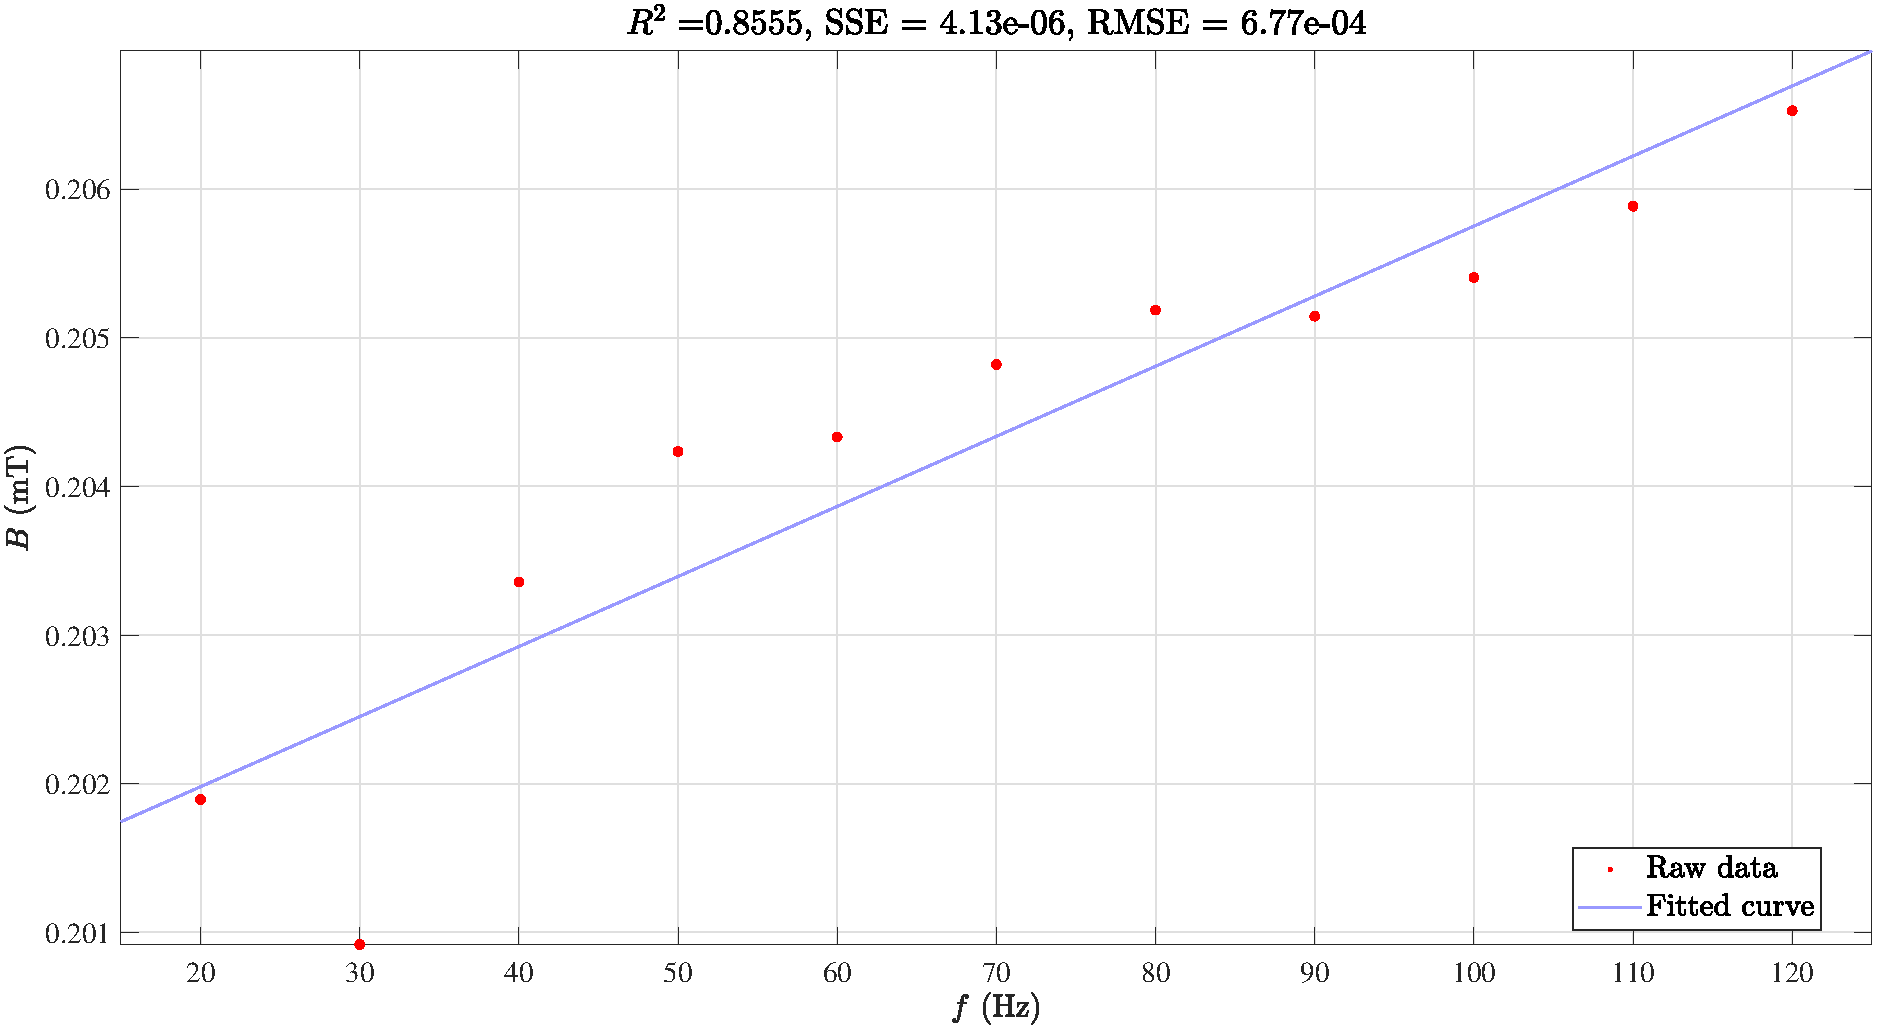
\includegraphics[width=0.9\columnwidth]{assets/2/10.pdf}
    \caption{励磁电流频率大小对磁场强度的影响}
\end{figure}
拟合斜率$ 4.713\times10^{-5} \ \mathrm{mT}\cdot \ \mathrm{Hz^{-1}}$ 远小于 $\boldsymbol{B}$ 测量值,因此在误差范围内可认为频率$ f $不影响磁场强度。

\newpage


\section{思考题}

\subsection*{3.1\ \ \ 第一部分思考题}
\subsubsection*{3.1.1\ \ 分析本实验主要误差来源,计算磁场$ B $的合成不确定度(分别取$ I_M=1.0\,\mathrm A,\;I_H=10\,\mathrm{mA} $)}

本实验误差除因实验器材本身损耗外,还来自于数字电流、电压表示数的精度,示数不稳定造成的读数误差等。我们有下面的已知量:
\begin{gather}
    K_H = 363.6 \  \  \ \mathrm{mV}\cdot \mathrm{A^{-1}}\cdot \mathrm{mT}^{-1},\quad \sigma_{K_H} = 0.8\ \mathrm{mV}\cdot \mathrm{A^{-1}}\cdot \mathrm{mT}^{-1} \\
    I_S = 1 \ \mathrm{mA},\quad \sigma_{I_S} = 1\times10^{-5} \ \mathrm{A} \\
    U_H = 25.7 \ \mathrm{mV},\quad \sigma_{U_H} = 1\times10^{-4} \ \mathrm{V}
\end{gather}
则有:
\begin{align}
    \sigma_B & =\sqrt{\left(\frac{\partial B}{\partial K_H}\sigma_{K_H}\right)^2+\left(\frac{\partial B}{\partial I_S}\sigma_{I_S}\right)^2+\left(\frac{\partial B}{\partial U_H}\sigma_{U_H}\right)^2}\\
    & =\sqrt{(I_SU_H\sigma_{K_H})^2+(I_S\sigma_{U_H}K_H)^2+(\sigma_{I_S}U_HK_H)^2}\\
    & = 0.1024 \,\mathrm{mT}
\end{align}


\subsubsection*{3.1.2\ \ 以简图示意,用霍尔效应法判断霍尔片上的磁场方向}
不妨令霍尔元件为长方体,如图 \ref{霍尔效应原理示意图(正电荷,空穴型)} 所示。若将通有电流的导体置于磁场 $\boldsymbol{B}$ 之中,磁场 $\boldsymbol{B}$ (沿$ z $轴)垂直于电流$ I_S $(沿$ x $轴)的方向,如下图所示,那么在导体中垂直于 $\boldsymbol{B}$ 和$ I_S $的方向上出现一个横向电位差$ U_H $,磁场、电势差和电流之间的方向关系已在图中标出。
\begin{figure}[H]
    \centering
    \begin{tikzpicture}
        \draw (0,0) rectangle (4,1);
        \draw (4,0)--(6,2)--(6,3)--(4,1)--cycle;
        \draw (0,1)--(2,3)--(6,3);
        \draw[dashed] (0,0)--(2,2)--(6,2);
        \draw[dashed] (2,2)--(2,3);
        \node at(2,0.5) {$ ++++++++ $};
        \node at(4,2.5) {$ -------- $};
        \draw[->] (-2,1.5)node[left]{1}--node[above,midway]{$ I_S $}(0.3,1.5);
        \draw (3,1.5)node{$ + $} circle (0.2);
        \draw[->] (2.859,1.359)--(2.577,1.077)node[left]{$ F_B $};
        \draw[->] (3.141,1.641)--(3.441,1.941)node[right]{$ F_E $};
        \draw[->] (3.2,1.5)--(4,1.5)node[right]{ $\boldsymbol{v}$ };
        \draw[->] (3,3.5)--(3,4.5)node[above]{$ B $};
        \draw (4.1,0)--(4.9,0);
        \draw (6.1,2)--(6.9,2);
        \draw (6.1,3)--(6.9,3);
        \draw[<->] (4.5,0)--node[right,midway]{$ w $}(6.5,2);
        \draw[<->] (6.5,2)--node[right,midway]{$ d $}(6.5,3);
        \draw[->] (5,1.5)--(7.5,1.5)node[right]{2};
        \draw (2,0.3)--(1.7,-0.5)node[below]{3};
        \draw (4.5,3)--(4.8,3.4)node[above right]{4};
        
        \draw[->] (9,-1)--(9,1)node[above]{$ z $};
        \draw[->] (9,-1)--(10.414,0.414)node[above right]{$ y $};
        \draw[->] (9,-1)--(11,-1)node[right]{$ x $};
    \end{tikzpicture}
    \caption{霍尔效应原理示意图(正电荷,空穴型)}
    \label{霍尔效应原理示意图(正电荷,空穴型)}
\end{figure}


\subsubsection*{3.1.3\ \ 如何测量交变磁场,写出主要步骤}
可以对示波器所得数据进行积分,得到磁感应强度大小。主要步骤为:
\begin{enumerate}
\item 将霍尔元件置于交变磁场中;
\item 利用交变磁场激励一个探测线圈,并将线圈接在示波器上,转动线圈至电动势达到最大值,这一步是为了保证垂直;
\item 已知线圈匝数$ N $、面积$ S $,则可利用感生电动势公式 $ E=NS\frac{\ \mathrm{d} B}{\ \mathrm{d} t} $ 对波形曲线作积分以得到交变磁场中磁感应强度与时间的关系式;
\item 由关系式求出磁感应强度大小 $B$。
\end{enumerate}

\subsection*{3.2\ \ \ 第二部分思考题}
\subsubsection*{3.2.1\ \ 单线圈轴线上磁场的分布规律如何?亥姆霍兹线圈是怎样组成的?其基本条件有哪些?它的磁场分布特点怎样?}
圆线圈轴线上的磁场分布为:
\begin{equation}\label{单线圈轴线上磁场分布}
B = \frac{\mu_0}{4 \pi} \oint_L \frac{I\sin \theta \ \mathrm{d} l}{r^2} = \frac{\mu_0 I}{2}\cdot \frac{R^2}{\left( R^2 + x^2 \right)^{\frac{3}{2}}}
\end{equation}
上式表明,磁感应强度在轴线中点处最大 $B_{\max} = \frac{\mu_0 I}{2 R}$,从中心位置向两侧递减,且两侧分布对称。

亥姆霍兹线圈是一对共轴平行放置、线圈间距 $a$ 等于线圈半径 $R$、通以同方向电流、参数一致的圆线圈。亥姆霍兹线圈的总磁场在轴线中点或径向中点处附近一定范围内均匀分布。只需将公式 (\ref{单线圈轴线上磁场分布}) 中的 $x$ 分别变换为 $x + \frac{R}{2}$ 和 $x - \frac{a}{2}$,即可得到磁场分布:
\begin{equation}
    B=\frac12\mu_0NIR^2\left\{\left[R^2+\left(z + \frac R2\right)^2\right]^{-3/2}+\left[R^2+\left(z - \frac R2\right)^2\right]^{-3/2}\right\} 
\end{equation}

\subsubsection*{3.2.2\ \ 探测线圈放入磁场后,不同方向上毫伏表指示值不同,哪个方向最大?如何测准$ U_{\max} $值?指示值最小表示什么?}
当磁感应强度方向与探测线圈平面垂直,即探测线圈轴线方向与磁感应线方向平行时,磁通量变化率最大,毫伏表的指示值最大。为测量$ U_{\max} $值,可分别测量该位置下$ \theta=0^\circ $与$ 180^\circ $时的值,取其平均值作为测量结果。

指示值最小意味着在该方向上,磁通量变化率最小,磁感应强度方向与探测线圈平面几乎平行,即与探测线圈轴线方向几乎垂直。

\subsubsection*{3.2.3\ \ 分析圆电流磁场分布的理论值与实验值的误差的产生原因}
从模型的角度来讲,一方面,实际的圆线圈是有直径的,不能看作直径为 0(极细)的理想圆线圈;另一方面,探测线圈并非质点,测试结果与理想模型间存在差异。从测量的角度来讲,实验设备的损耗等因素使得实验器材实际参数与计算所用参数间存在偏差,此外数据采集时读数、跳变、精度等也可能造成一定的实验误差。

\section{实验总结与心得体会}
此次“磁场测量”实验共分为两个部分,总的来讲都是依据磁场与霍尔效应的特性来设计实验,测出磁场或霍尔效应相关参量,并与理论值(标准值)作对比。实验的一大重点是“对称交换法消除系统误差”,令我印象深刻;另一重点是数据的计算、拟合与不确定度分析,在处理的过程中,我也学到很多。

实验总体上是成功的,每个小节的实验都大致符合理论,实验数据和图像也具有较强的说服力。例如霍尔灵敏度 $K_H$ 的实验测量值与仪器标准值误差仅为 $-1.98 \%$。

特别地,在本次实验,我利用了 Matlab 软件对实验数据作进一步的处理和分析,包括换算、拟合、可视化等,相比于常规数据处理和画图方法,这大大提高了数据分析处理的速度的准确度,也提高了作图的美观性。在今后的实验和研究工作中,我还会继续深入学习和应用类似地计算软件,增强自己的科学计算能力。科研不是考试,我们应该充分利用好自己能接触到的资源,合理使用工具,更高效地发展自身。

另外,这次实验让我感受到,实验“结束”并不意味着实验就已经完成,事实上这仅是数据测量的结束。在课后,我们还需要重新整理实验原理和过程,换算、分析、拟合实验数据,作出合适的数据图,解释可能存在的误差等。在根据已有数据求所需结果时,如何才能最大程度地利用已有数据,同时又尽可能地降低二次误差。上面这些内容都需要体现在最终的实验报告中,一点点累加起来,着实花费了我很多精力。

但最后回过头来,我认为一切都是值得的。当处理完毕的结果有力地验证了理论值时,当实验数据图像与理论较好地契合时,心中便迸发出无尽的喜悦,也深深感受到物理“理论与实验结合”的魅力\footnote{手写预习报告、原始数据记录表和 Matlab 源码附在附录中。}。

\newpage
\section*{附录 A\hspace*{20pt} 原始数据记录表}
\addcontentsline{toc}{section}{附录 A\hspace*{6pt} 原始数据记录表} 
\thispagestyle{fancy} 

\begin{figure}[H]\centering
    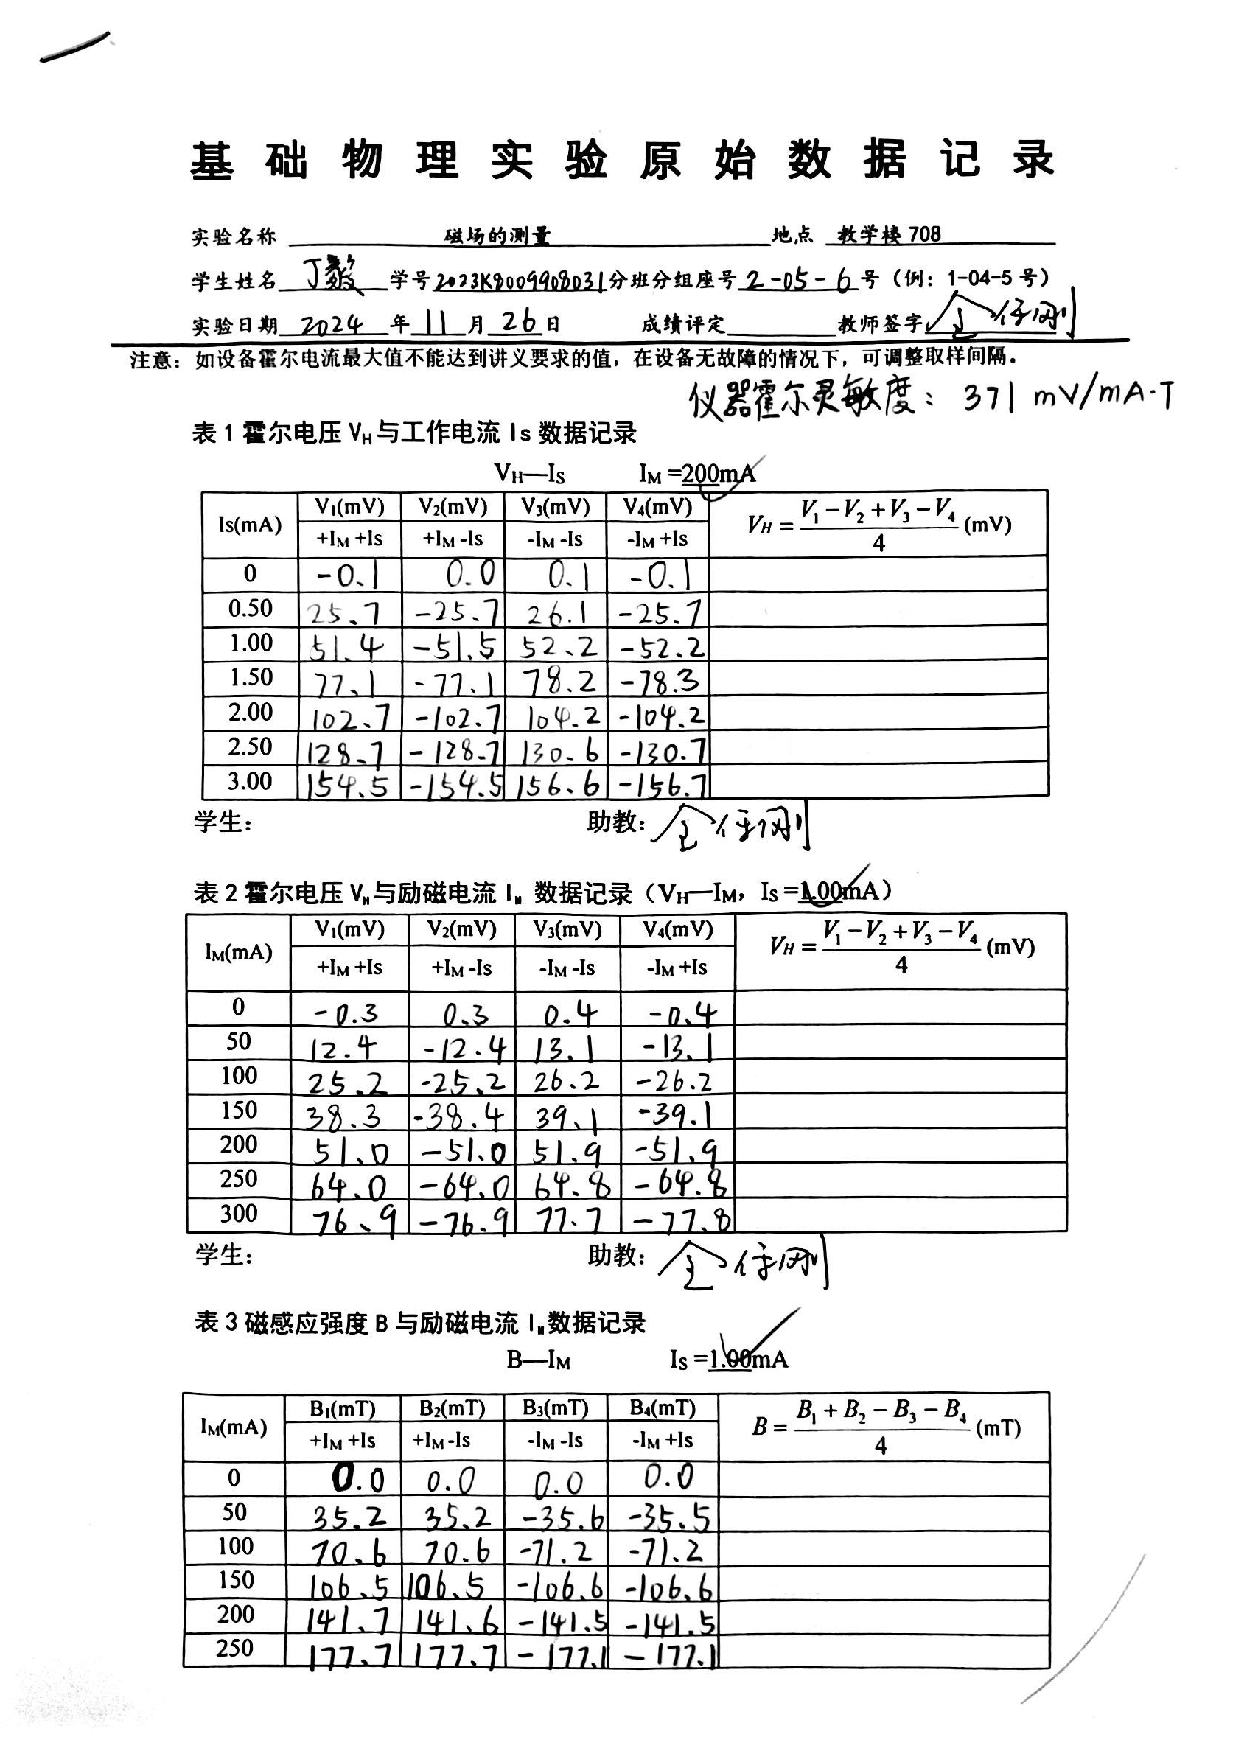
\includepdf[pages=1, width=480pt]{pdf/原始数据-2-05组-丁毅-磁场测量-2024.11.26-全保刚.pdf}
\end{figure}
\includepdf[pages={2}]{pdf/原始数据-2-05组-丁毅-磁场测量-2024.11.26-全保刚.pdf}

\section*{附录 B\hspace*{20pt} 手写预习报告}
\addcontentsline{toc}{section}{附录 B\hspace*{6pt} 手写预习报告} 
\thispagestyle{fancy} 

\begin{figure}[H]\centering
    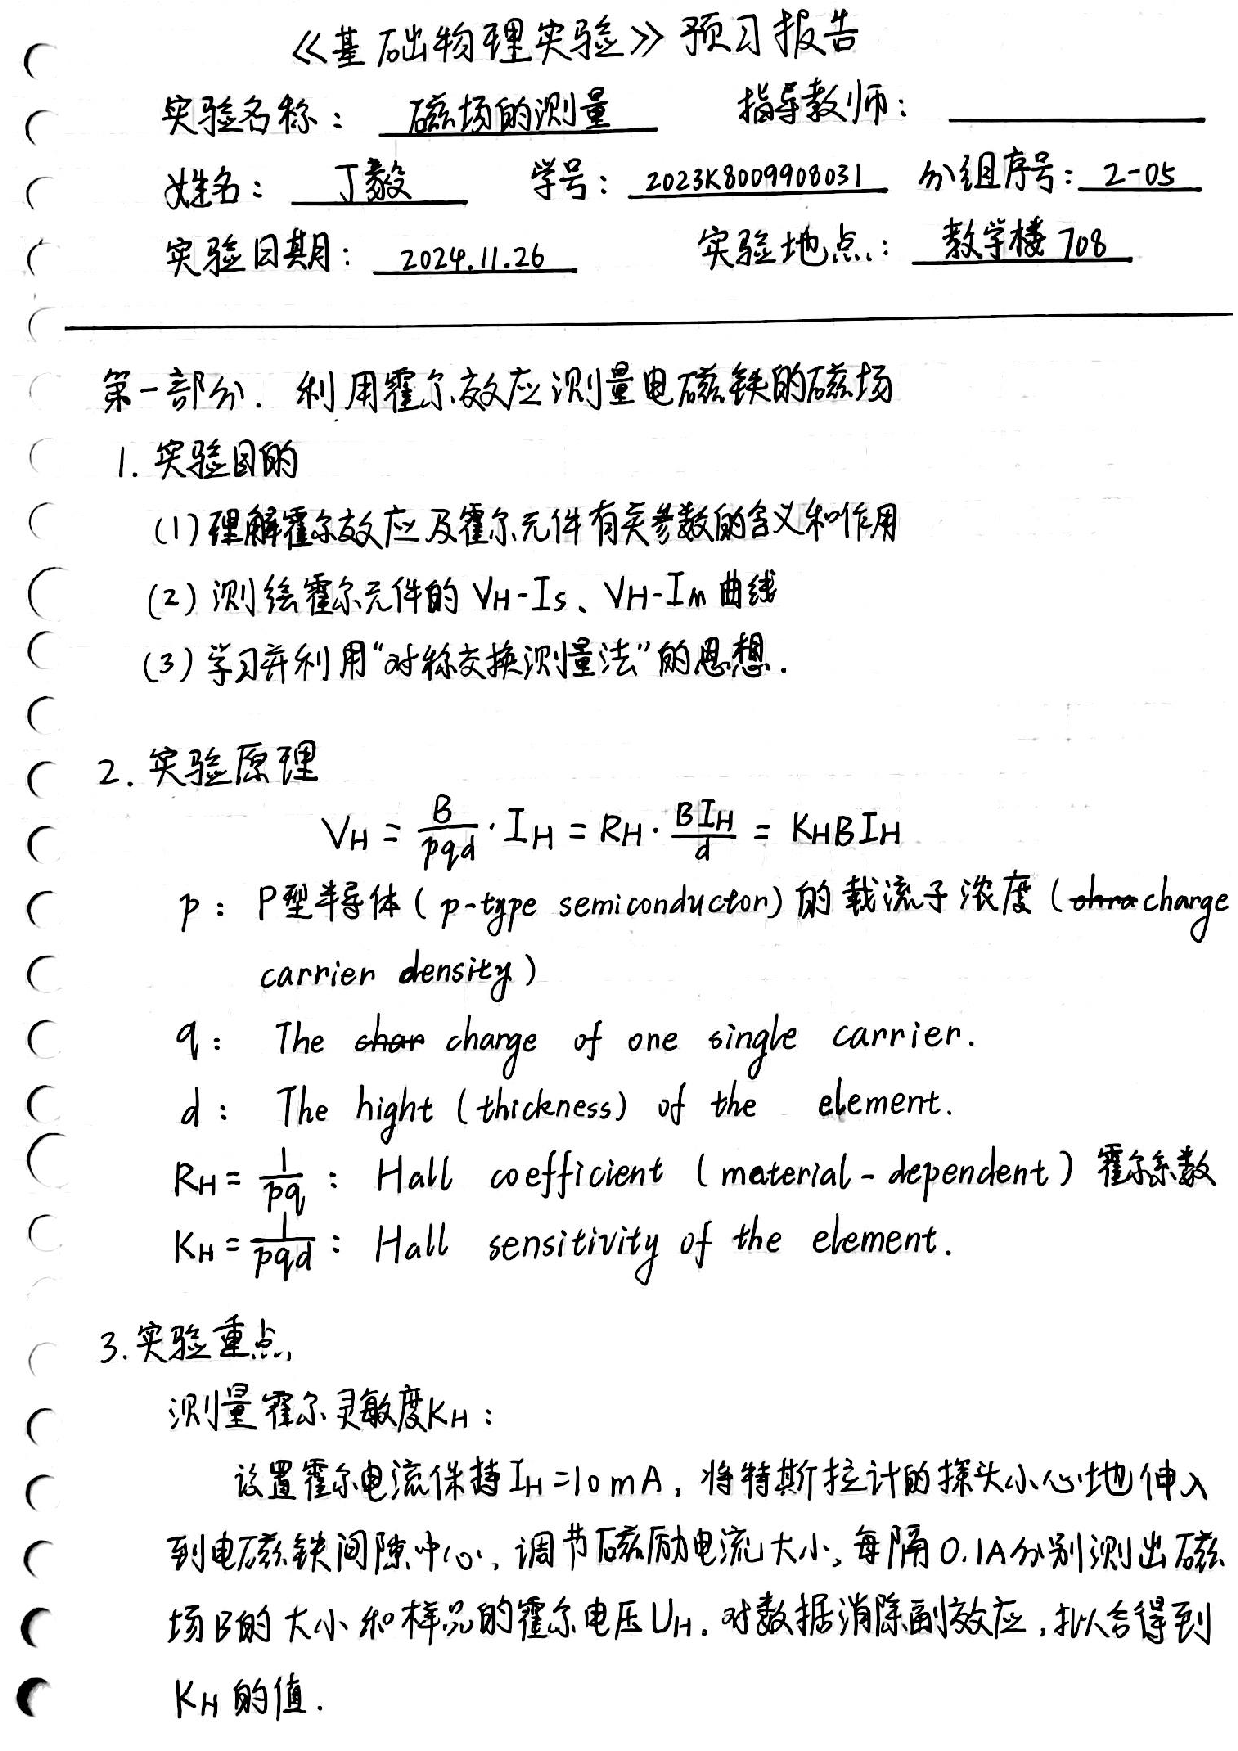
\includepdf[pages=1, width=480pt]{pdf/预习报告-2-05组-丁毅-磁场测量-2024.11.26-全保刚.pdf}
\end{figure}
\includepdf[pages={2}]{pdf/预习报告-2-05组-丁毅-磁场测量-2024.11.26-全保刚.pdf}

\section*{附录 C\hspace*{20pt} Matlab 源码}
\addcontentsline{toc}{section}{附录 C\hspace*{6pt} Matlab 源码} 
\thispagestyle{fancy} 
\lstinputlisting{d:/a_RemoteRepo/GH.MatlabCodes/本科课程代码/基础物理实验/Ex_2/Ex_02_mfile.m}



\end{document}

% VScode 常用快捷键:

% F2:                       变量重命名
% Ctrl + Enter:             行中换行
% Alt + up/down:            上下移行
% 鼠标中键 + 移动:           快速多光标
% Shift + Alt + up/down:    上下复制
% Ctrl + left/right:        左右跳单词
% Ctrl + Backspace/Delete:  左右删单词    
% Shift + Delete:           删除此行
% Ctrl + J:                 打开 VScode 下栏(输出栏)
% Ctrl + B:                 打开 VScode 左栏(目录栏)
% Ctrl + `:                 打开 VScode 终端栏
% Ctrl + 0:                 定位文件
% Ctrl + Tab:               切换已打开的文件(切标签)
% Ctrl + Shift + P:         打开全局命令(设置)

% Latex 常用快捷键:

% Ctrl + Alt + J:           由代码定位到PDF


